%
% chapter.tex -- Affine Vektorgeometrie
%
% (c) 2018 Prof Dr Andreas Müller, Hochschule Rapperswil
%
\chapter{Affine Vektorgeometrie\label{chapter:affin}}
Mit den in Kapitel~\ref{chapter-lingl} entwickelten Methoden zur Lösung
linearer Gleichungen und den algebraischen Konzepten von Matrizen und Vektoren
können auch geometrische Situationen effizient beschrieben werden.
Dazu benötigt man zunächst Beschreibung des geometrischen Raumes mit Hilfe von
Vektoren.
Dazu dient das Konzept der Basis und des zugehörigen Koordinatensystems,
welches in Abschnitt~\ref{section:basis} eingeführt wird.
Da der gleiche geometrische Raum mit verschiedenen Koordinatensystemen
beschrieben werden kann, müssen wir im Golgenden immer auch untersuchen,
wie sich die Beschreibung eines geometrischen Objektes ändert, wenn man
eine andere Basis verwendet.

In Abschnitt~\ref{section:lineare abbildungen} wird gezeigt, wie sich
geometrische Abbildungen als lineare Abbildungen verstehen lassen und
daher mit Hilfe von Matrizen beschreiben lassen.
Das Matrizenprodukt erhält damit eine anschauliche Bedeutung als die
Komposition von Abbildungen.

Geraden und Ebenen sowie höherdimensionale Unterräume von Vektorräumen
können alle mit Hilfe von linearen Abbildungen beschrieben.
Probleme der Lage wie zum Beispiel die Existenz und Eindeutigkeit von
Schnittpunkten von solchen Objekten wird damit auf algebraische Probleme
mit Matrizen und linearen Gleichungssytemen zurückgeführt.
Das Ziel von Abschnitt~\ref{section:alggeo} ist daher, eine Technik
zur Übersetzung von geometrischen Problemen in algebraische zu finden,
so dass der Gauss-Algorithmus von Kapitel~\ref{chapter-lingl} zum universellen
Lösungsalgorithmus für solche Problem wird.

In diesem Kapitel begnügen wir uns mit den in Kapitel~\ref{chapter-lingl}
entwickelten Konzepten.
Insbesondere kennen wir noch kein Konzept für Längen, Winkel,
Flächeninhalte oder Volumina.
Diese erfordern als zusätzliche Struktur das Skalarprodukt, welches in
Kapitel~\ref{chapter:orthogonalitaet} eingeführt wird, oder die Orientierung,
welche Kapitel~\ref{chapter:orientierung} zum ermöglich das Vektorprodukt
zu definieren.

\begin{verbatim}
5.1 Determinante und Orientierung
- Orientierter Flächeninhalt
- Orientiertes Volumen
5.2 Vektorprodukt
- Definition und Eigenschaften
- Normalenvektoren
- Abstandsformeln
\end{verbatim}



%
% koordinatensysteme.tex
%
% (c) 2018 Prof Dr Andreas Müller, Hochschule Rapperswil
%
\section{Punkte und Koordinatensysteme}
\subsection{Punkte im Raum und Vektoren}
\subsubsection{Koordinatensystem}
Punkte der Ebene können mit Hilfe eines Koordinatensystems festgelegt
werden: von einem Ausgangspunkt $O$, dem Nullpunkt des Koordinatensystems
aus, werden die Koordinaten entlang zweier aufeinander senkrecht stehender
Richtungen, den Achsrichtungen abgetragen.
Die Geraden durch den Ursprung
des Koordinatensystems in Achsrichtung heissen die Koordinatenachsen.

\begin{figure}
\begin{center}
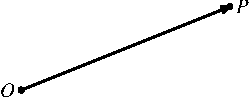
\includegraphics{images/v-1}
\end{center}
\caption{Vektor zwischen zwei Punkten $O$ und $P$, Ortsvektor des Punktes $P$
\label{image-vektor}}
\end{figure}
Ein Punkt $P$ wird durch die Länge der Projektionen der Strecke $OP$
auf die Achsrichtungen festgelegt, also durch ein Zahlenpaar $(x,y)$.
Der Punkt $(1,0)$ liegt auf der $x$-Achse, eine Einheit vom Punkt $O$
entfernt.
Der Punkt $(0,1)$ liegt gleich weit entfernt von $O$ auf der $y$-Achse.

\subsubsection{Ortsvektoren}
Die Einführung eines Koordinatensystems ermöglicht zwar, Punktmengen
in der Ebene durch algebraische Beziehungen zwischen den Koordinaten
zu beschreiben, zum Beispiel ist der Einheitskreis die Menge der
Punkte
\[
\{(x,y)\;|\;x^2+y^2=1\}.
\]
``Rechnen'' kann man mit den Punkten aber noch nicht.
Dazu bilden wir
die Spaltenvektoren, mit denen wir ja bereits zu rechnen gelernt haben,
wie folgt auf die Punkte der Ebene ab:
\[
\begin{pmatrix}x\\y\end{pmatrix}
\mapsto (x,y)
\]
Den Vektor $\begin{pmatrix}x\\y\end{pmatrix}$ können wir uns als
Vektor vom Nullpunkt des Koordinatensystems zum Punkt $P=(x,y)$ vorstellen:
\[
\begin{pmatrix}x\\y\end{pmatrix}
=
\overset{\rightarrow}{OP}.
\]
\index{Ortsvektor}
$\overrightarrow{OP}$ heisst
heisst {\em Ortsvektor} des Punktes $P$.
Analoges gilt in drei Dimensionen:
\[
\begin{pmatrix}x\\y\\z\end{pmatrix}
\mapsto
(x,y,z)
\]
Ja es gibt überhaupt keinen Grund, die Geometrie auf zwei oder drei
Dimensionen zu beschränken, wir können Vektoren beliebiger Dimension
auf Punkte
abbilden, die entsprechend viele Koordinaten haben:
\[
\begin{pmatrix}
x_1\\x_2\\\vdots\\x_n
\end{pmatrix}
\mapsto
(x_1,x_2,\dots,x_n)
\]

\subsubsection{Vektoroperationen}
Die Rechenoperationen mit Vektoren können wir ebenfalls in geometrische
Begriffe übersetzen:
\begin{figure}
\begin{center}
\begin{tabular}{cc}
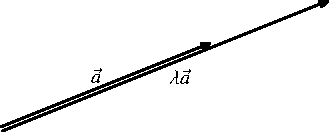
\includegraphics{images/v-2}&
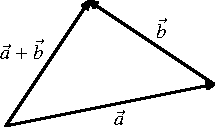
\includegraphics{images/v-3}
\end{tabular}
\end{center}
\caption{Algebraische Operationen mit Vektoren\label{image-vektor-operationen}}
\end{figure}
\begin{itemize}
\index{Streckung}
\item Die Multiplikation mit einer Zahl $\lambda$ ist eine Streckung mit
Zentrum $O$ und Streckfaktor $\lambda$.
\index{Aneinandersetzen}
\item Die Addition von zwei Vektoren entspricht dem ``Aneinandersetzen''
der Strecken.
\end{itemize}
\begin{figure}
\begin{center}
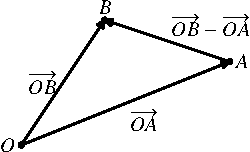
\includegraphics{images/v-4}
\end{center}
\caption{Vektor $\overset{\rightarrow}{AB}$
\label{image-vektorab}}
\end{figure}
Besonders im Falle der Addition spielt die ``Richtung'' der Strecken eine
Rolle, wir symbolisieren diese Richtung durch einen Pfeil.
Der Pfeil vom Punkt $A$ zum Punkt $B$ ist die Differenz der Vektoren die von
$O$ zum Punkt $B$ bzw.~zu $A$ führen:
\[
\overset{\rightarrow}{AB}=\overset{\rightarrow}{OB}-\overset{\rightarrow}{OA}
\]

\subsubsection{Vektoren als Translationen}
Vektoren können auch als Verschiebungs-Operationen  oder Translationen
des Raumes betrachtet werden.
Wenn eine Verschiebung den Punkt $A$ in den Punkt $B$ verschiebt,
verschiebt sie den Punkt $C$ in den Punkt $D$ mit Ortsvektor
\[
\overrightarrow{OD}
=
\overrightarrow{OC}+\overrightarrow{AB}
=
\overrightarrow{OC}+\overrightarrow{OB}-\overrightarrow{OA}.
\]
Die Verschiebung entspricht also der Addition eines Verschiebungsvektors
zu allen Ortsvektoren.

\subsubsection{Bemerkungen zur Notation}
In diesem geometrischen Zusammenhang werden wir oft Vektoren als
kleine Buchstaben mit einem Pfeil schreiben: $\vec v$.
Um jedoch interessante
Geometrie zu treiben, müssen wir die üblichen geometrischen Begriffe in
Vektorschreibweise übersetzen: Geraden, Ebenen, Kreise, Kugeln.
Ausserdem müssen wir lernen, wie übliche geometrische Konstruktionen in
Rechenoperationen mit Vektoren übersetzt werden können.

\subsection{Basis}
\index{Basis}
\begin{figure}
\begin{center}
%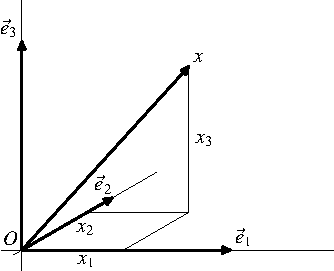
\includegraphics{images/v-5}
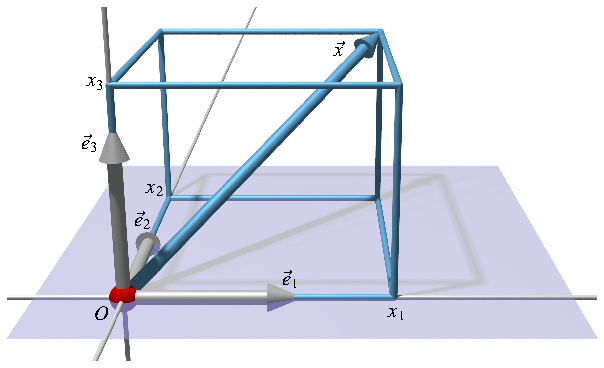
\includegraphics{3/images/coordsystem.pdf}
\end{center}
\caption{Darstellung des Vektors $\vec{x}$ in der Basis
$\{\vec{e}_1,\vec{e}_2,\vec{e}_3\}$ als
$\vec{x} =
x_1\vec{e}_1+
x_2\vec{e}_2+
x_3\vec{e}_3$.
\label{imagebasis}}
\end{figure}
Im Abschnitt \ref{speziellevektoren} haben wir die Vektoren $e_i$
kennengelernt.
Im aktuellen Zusammenhang schreiben wir dafür oft auch
\[
\vec e_1=\begin{pmatrix}1\\0\\0\end{pmatrix},\qquad
\vec e_2=\begin{pmatrix}0\\1\\0\end{pmatrix},\qquad
\vec e_3=\begin{pmatrix}0\\0\\1\end{pmatrix}.
\]
Diese Vektoren konnten dafür verwendet werden, einen beliebigen Vektor
mit Hilfe einer Linearkombination zusammenzusetzen:
\[
\vec v=
v_1\vec e_1+
v_2\vec e_2+
v_3\vec e_3.
\]
Die speziellen Vektoren $e_1,\dots,e_n$ sind nicht die einzig möglichen,
mit denen man die Position eines Punktes auf vektorielle Weise
beschreiben könnte.
Jeder andere Satz von $n$ Vektoren kann
dazu verwendet werden, sofern sich damit jeder beliebige Vektor
linear kombinieren lässt.
In Kapitel~1 haben wir gelernt, dass dies
gleichbedeutend damit ist, dass die Vektoren linear unabhängig sein
müssen.
\begin{definition}
$n$ linear unabhängige Vektoren $b_1,\dots,b_n$ heissen eine
Basis des $n$-dimensionalen Raumes.
\end{definition}
Um die Koordinaten eines Punktes $x$ in dieser Basis zu bestimmen,
müssen die Zahlen $\xi_1,\dots,\xi_n$ berechnet werden für die
gilt
\[
b_1\xi_1+\dots+b_n\xi_n=x.
\]
Ausgeschrieben ist dies das Gleichungssystem
\[
\begin{linsys}{3}
b_{11}\xi_1&+&\dots &+&b_{1n}\xi_n&=&x_1\\
\vdots   & &\ddots& &\vdots&&\vdots\\
b_{n1}\xi_1&+&\dots &+&b_{nn}\xi_n&=&x_n\\
\end{linsys}
\]
Sind die Vektoren linear unabhängig, dann ist die Koeffizientenmatrix
regulär, das Gleichungssystem hat also genau eine Lösung.
Die behauptete Darstellung ist also immer möglich.

Somit haben wir eine weitere Interpretation einer regulären Matrix:
die Spalten einer regulären Matrix sind Vektoren, die man dazu verwenden
kann, jeden beliebigen anderen Vektor linear zu kombinieren.

\begin{beispiel}
Man stelle den Vektor $\vec v$ in der Basis $b_1,b_2,b_3$ dar:
\[
\vec b_1=\begin{pmatrix}2\\-3\\-2\end{pmatrix},\quad
\vec b_2=\begin{pmatrix}6\\-2\\-3\end{pmatrix},\quad
\vec b_3=\begin{pmatrix}-1\\2\\1\end{pmatrix},\qquad
\vec v=\begin{pmatrix}-6\\3\\3\end{pmatrix}.
\]

\smallskip

{\parindent 0pt
Die} Koordinaten $(\xi_1,\xi_2,\xi_3)$ müssen gefunden
werden, so dass
\[
\xi_1\vec b_1+
\xi_2\vec b_2+
\xi_3\vec b_3
=
\vec v,
\]
d.~h.
\[
\xi_1\begin{pmatrix}2\\-3\\-2\end{pmatrix}+
\xi_2\begin{pmatrix}6\\-2\\-3\end{pmatrix}+
\xi_3\begin{pmatrix}-1\\2\\1\end{pmatrix}=
\begin{pmatrix}-6\\3\\3\end{pmatrix}
\quad
\Leftrightarrow
\quad
\begin{pmatrix}
2&6&-1\\
-3&-2&2\\
-2&-3&1
\end{pmatrix}
\begin{pmatrix}\xi_1\\\xi_2\\\xi_3\end{pmatrix}
=
\begin{pmatrix}-6\\3\\3\end{pmatrix}.
\]
Auflösung des Gleichungssystems mit dem Gauss-Algorithmus oder mit
dem Computer ergibt.
\[
\begin{pmatrix}\xi_1\\\xi_2\\\xi_3\end{pmatrix}
=
\begin{pmatrix}1\\-1\\2 \end{pmatrix}.
\]
\end{beispiel}


%
% basis.tex
%
% (c) 2017 Prof Dr Andreas Müller, Hochschule Rapperswil
%
\section{Basis}
Der $K$-Vektorraum $K[X]$ hat die Eigenschaft, dass jeder Vektor darin,
also jedes Polynom mit Koeffizienten $K$ als Linearkombination einer
kleinen Menge von Vektoren geschrieben werden kann.
Die Monome
\[
\begin{aligned}
p_0(X)&=1,
&
p_1(X)&=X,
&
p_2(X)&=X^2,
&&\dots&
p_n(X)&=X^n,
&&\dots
\end{aligned}
\]
Das Polynom $p(X)=a_0+a_1X+a_2X^2+\dots+a_nX^n$ ist die Linearkombination
\[
p(X)
=
a_0p_0(X)
+
a_1p_1(X)
+
a_2p_2(X)
+\dots
+
a_np_n(X).
\]
Nach dem Prinzip des Koeffizientenvergleichs
ist ausserdem die Darstellung von $p(X)$ als Linearkombination
der Polynome $p_0,p_1,\dots,p_n,\dots$ eindeutig.
Die Menge
\[
B=\{p_0,p_1,\dots,p_n,\dots\}
\]
hat eine spezielle Bedeutung für den Vektorraum $K[X]$, jeder Vektor
von $K[X]$ lässt sich auf genau eine Weise als Linearkombination der
Vektoren aus $B$ darstellen.
Da die Darstellung immer eindeutig ist, sind die Vektoren in $B$
linear unabhängig.
Da sich jeder Vektor als Linearkombination darstellen lässt, ist
$K[X]=\langle B\rangle$.

\begin{definition}
Eine Teilmenge $B\subset V$ von Vektoren eines $K$-Vektorraums heisst
eine {\em Basis} von $V$, wenn jeder Vektor $v\in V$ auf genau eine Art
als Linearkombination
\[
v=\lambda_1b_1+\dots+\lambda_nb_n
\]
von Vektoren $b_1,\dots,b_n\in B$ dargestellt werden kann.
\end{definition}

Man beachte, dass nicht gefordert wurde, dass die Menge $B$ endlich sein
muss.
Es ist aber aus der Definition klar, dass die Vektoren in $B$ linear
unabhängig sind und zusammen den ganzen Vektorraum erzeugen,
also $V=\langle B\rangle$.

\begin{definition}
Ein Vektorraum $V$ heisst {\em endlichdimensional}, wenn er eine Basis $B$
mit endlich vielen Vektoren besteht.
Die {\em Dimension} eines endlichdimensionalen Vektorraums $V$ ist
die Anzahl der Basisvektoren $\operatorname{dim} V = |B|$.
\end{definition}

Diese Definition ist nur sinnvoll, wenn alle möglichen Basen von $V$ die
gleiche Anzahl Basisvektoren haben, dies ist aber nicht unmittelbar klar.
Wir fassen das in die Form eines Lemmas und formulieren einen abstrakten
formalen Beweis.

\begin{lemma}
Sei $V$ ein endlichdimensionaler $K$-Vektorraum, dann hat jede Basis
von $V$ die gleiche Anzahl Basisvektoren.
\end{lemma}

\begin{proof}[Beweis]
Seien $B$ und $\tilde B$ zwei verschiedenen Basen mit Basisvektoren
$b_1,\dots,b_n\in B$ und $\tilde b_1,\dots,\tilde b_m\in \tilde B$,
wobei wir ohne Einschränkung der Allgmeinheit annehmen dürfen, dass $n>m$
ist.
Da sowohl $B$ als auch $\tilde B$ Basen sind, lässt sich jeder Basisvektor
aus den jeweils anderen Basisvektoren linear kombinieren.
Es gibt also eindeutig bestimmte Zahlen $a_{ij}\in K$ und
$\tilde a_{ij}\in K$ mit
\[
\tilde b_j = \sum_{i=1}^n a_{ji} b_i
\qquad\text{und}\qquad
b_i = \sum_{j=1}^m \tilde a_{ij}\tilde b_j.
\]
Wir behaupten, dass die Vektoren $b_1,\dots,b_n$ linear abhängig sein 
müssen, dass also $B$ gar keine Basis sein kann.

Wir behaupten also, dass es Zahlen $\lambda_1,\dots,\lambda_n\in K$
gibt mit der Eigenschaft
\[
\lambda_1 b_1+\dots+\lambda_n b_n = 0,
\]
wir müssen zeigen, wie man die Zahlen $\lambda_i$ finden kann.
Setzt man die Darstellung durch die Vektoren $\tilde b_j$ ein, erhält man
\[
\sum_{i=1}^n
\lambda_i
\sum_{j=1}^m
\tilde a_{ij}\tilde b_j
=
\sum_{j=1}^m
\biggl(
\sum_{i=1}^n
\lambda_i
\tilde a_{ij}
\biggr)
\tilde b_j
=
0.
\]
Da die Vektoren $\tilde b_j$ linear unabhängig sind, muss in dieser
Summe jede Klammer verschwinden:
\[
\sum_{i=1}^n \tilde a_{ij}\lambda_i =0 
\]
Dies ist ein lineares Gleichungssystem mit $m$ Gleichungen ($j=1,\dots,m$)
für $n$ Unbekannte ($i=1,\dots,n$).
Aus der elementaren Theorie wissen wir, dass ein solches Gleichungssystem
eine nichttriviale Lösung haben muss.
Damit ist gezeigt, dass die Vektoren $b\in B$ nicht linear unabhängig sein
können, $B$ kann also gar keine Basis sein.
Folglich müssen zwei Basen eines endlichdimensionalen Vektorraums
die gleiche Anzahl.
\end{proof}

\subsubsection{Spaltenvektoren}
Wir haben diesen formalen Beweis noch aus einem anderen Grund im
Detail durchgeführt.
Mit Hilfe der Basis haben wir das Problem auf eine Frage über ein
Gleichungssystem reduziert.
Dies ist ein allgemeines Prinzip.
Sei $B=\{b_1,\dots,b_n\}$ eine Basis des Vektorraums $V$.
dann lässt sich jeder Vektor $v\in V$  auf eindeutige Art als
Linearkombination von Vektoren von $B$ darstellen, es gibt
also Zahlen $v_i\in K$ mit der Eigenschaft
\[
v=v_1b_1+\dots+v_nb_n.
\]
Zu jedem Vektor $v\in K$ gibt es also einen Spaltenvektor mit Komponenten
$v_i$, die Abbildung
\[
\varphi\colon
V\to K^n
:
v\mapsto \begin{pmatrix}v_1\\\vdots\\v_n\end{pmatrix}
\]
ist eine lineare Abbildung.
Da jeder Vektor als Linearkombination von Vektoren aus $B$ geschrieben
werden kann, ist $\varphi$ surjektiv.
Weil die Darstellung als Linearkombination eindeutig ist, ist $\varphi$
auch injektiv.
$\varphi$ ist also ein bijektive lineare Abbildung $V\to K^n$.
Eine Basis ermöglich also, jeden beliebigen Vektorraum $V$ mit einem
Vektorraum $K^n$ von Spaltenvektoren zu identifizieren.

\subsubsection{Matrizen}
Seien jetzt $U$ und $V$ endlichdimensionale Vektorräume über dem Körper $K$ 
mit Basen $B=\{b_1,\dots,b_n\}$ bzw.~$C=\{c_1,\dots,c_m\}$.
Ausserdem sie $f\colon U\to V$ eine lineare Abbildung.
Dann kann jeder Vektor $f(b_i)\in V$ auf genau eine Weise als
Linearkombination von Vektoren aus $C$ dargestellt werden.
Es gibt also Zahlen $a_{ji}\in K$ derart, dass
\[
f(b_i) = \sum_{j=1}^m a_{ji}c_j.
\]
Sobald die $a_{ji}$ bekannt sind, lässt sich auch das Bild jedes
anderen Vektors $u\in U$ damit berechnen.
Der Vektor $u$ kann wie im vorangegangenen Abschnitt auf genau eine
Weise als Linearkombination der $b_i$ beschreiben, also
\[
u= u_1b_1+\dots+u_nb_n.
\]
Daraus ergibt sich jetzt
\[
f(u)
=
u_1f(b_1)+\dots+u_nf(b_n)
=
\sum_{i=1}^n  u_i \sum_{j=1}^m a_{ji}c_j
=
\sum_{j=1}^m \biggl(
\sum_{i=1}^n
a_{ji} u_i
\biggr) c_j
=
\sum_{j=1}^m v_jc_j.
\]
In der grossen Klammer stehen also die Komponenten $v_j$ von $f(u)$ in der
Basis $C$.
Wir haben also etabliert, dass die lineare Abbildung $f$ durch das
Matrizenprodukt
\[
\begin{pmatrix}
v_1\\\vdots\\v_m
\end{pmatrix}
=
\begin{pmatrix}
a_{11}&\dots&a_{1n}\\
\vdots&\ddots&\vdots\\
a_{m1}&\dots&a_{mn}
\end{pmatrix}
\begin{pmatrix}
u_1\\\vdots\\u_n
\end{pmatrix}
\]
wiedergeben wird.
Der Vektorraum der linearen Abbildungen von $U$ nach $V$ wird also
beschrieben durch den Vektorraum der $m\times n$-Matrizen mit
Einträgen in $K$.

Basen ermöglichen also nicht nur den Übergang von einem beliebigen
endlichdimensionalen Vektorraum zu einem Vektorraum von Spaltenvektoren,
sondern auch den Übergang vom Vektorraum der linearen Abbildungen 
zum Vektorraum der Matrizen.
Die Matrizen bilden also ein universelles Modell, auf das beliebige 
endlichdimensionale Vektorräume reduziert werden können.

Natürlich kann man aus Basen von $U$ und $V$ auch eine Basis von
$\operatorname{Hom}(U,V)$ konstruieren.
Die lineare Abbildung
\[
e_{ji}\colon U\to V:
b_k\mapsto \begin{cases}
c_j&\qquad i=k\\
0&\qquad i\ne k
\end{cases}
\]
hat die Matrix
\[
E_{ji}
=
\begin{pmatrix}
0     &\dots &0     &\dots &0     \\
\vdots&\ddots&\vdots&\ddots&\vdots\\
0     &\dots &1     &\dots &0     \\
\vdots&\ddots&\vdots&\ddots&\vdots\\
0     &\dots &0     &\dots &0     \\
\end{pmatrix}
\]
mit einer $1$ genau in Zeile $j$ und Spalte $i$ der Matrix.




%
% geraden.tex
%
% (c) 2018 Prof Dr Andreas Müller, Hochschule Rapperswil
%
\section{Geraden}
\rhead{Geraden}
\begin{figure}
\begin{center}
\begin{tabular}{ccc}
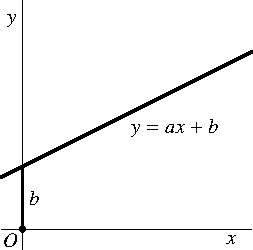
\includegraphics{images/v-6}&%
\qquad\qquad\qquad&
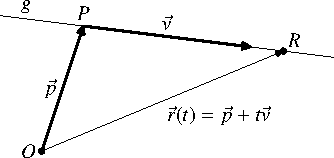
\includegraphics{images/v-7}%
\end{tabular}
\end{center}
\caption{Gerade in der Ebene (links) und Parametrisierung von Geraden im
Raum (rechts) \label{image-gerade}}
\end{figure}
Eine Gerade in einem Koordinatensystem in der Ebene kann durch eine
Gleichung der Form
\[
y=ax+b
\]
beschrieben werden (Abbildung~\ref{image-gerade}).
Die Gleichung hat als Lösungsmenge die Punkte
$(x,y)$, die auf einer Geraden der Steigung $a$ durch den Punkt $(0,b)$
liegen.
Der Nachteil dieser Darstellung ist, dass sich Geraden parallel zur $y$-Achse
damit nicht abbilden lassen.
Solche Geraden haben die Gleichung $x=c$, sie haben
``unendlich'' grosse Steigung.
Eine weitere Schwierigkeit besteht im Raum, wo noch eine weiter Koordinate
festzulegen ist.
Auch diese ist mit einer einzigen Gleichung nicht möglich.
Wir benötigen daher eine neue Form der Geradengleichung, welche für beliebige
Geraden in beliebigen Richtungen durch beliebige Punkte in beliebigen Räumen
unabhängig von der Dimension funktionieren.

\subsection{Parameterdarstellung}
\index{Parameterdarstellung!einer Gerade}
Die Punkte einer Geraden entstehen dadurch, dass ein Ausgangspunkt um
variable Längen in immer die gleiche Richtung verschoben wird.
Dies übersetzen wird jetzt in die Vektorsprache.
Eine Gerade wird also beschrieben durch
\begin{itemize}
\item einen Ausgangspunkt, oder seinen Ortsvektor $\vec p$.
Dieser Vektor heisst oft auch {\em Stützvektor}.
\index{Stutzvektor@Stützvektor}
\item Von diesem Ausgangspunkt aus müssen Strecken in eine bestimmte
Richtung angesetzt werden, dazu brauchen wir einen Vektor, wir nennen ihn
$\vec v$, den {\em Richtungsvektor}.
\index{Richtungsvektor}
\item Die angesetzten Vektoren sind von variabler Länge, es braucht also
einen Parameter, den wir $t\in \mathbb R$ nennen, mit welchem $\vec v$
multipliziert wird.
\end{itemize}
Auf diese Weise erreichen wir die Punkte $\vec r$ der Gerade mit Hilfe
einer Addition:
\[
\vec r(t)=\vec p+t\vec v,
\]
Abbildung~\ref{image-gerade}, rechts.
Mit dieser Definition lassen sich gewisse Grundaufgaben bereits lösen.

\begin{beispiel}
Man finde die Parameterdarstellung der Geraden durch die Punkte
$A=(3,1,4)$ und $B=(1,5,9)$.

\smallskip

{\parindent 0pt
Dazu} braucht man einen Vektor, der die Funktion von $\vec p$ übernehmen
kann, wir verwenden $\overrightarrow{OA}$ dafür, und als
Richtungsvektor können wir $\overrightarrow{AB}$ verwenden.
Damit wird die Geradengleichung
\begin{equation}
\vec r(t) =
\begin{pmatrix}3\\1\\4 \end{pmatrix}
+t
\begin{pmatrix}-2\\4\\5\end{pmatrix}.
\label{pigerade}
\end{equation}
\end{beispiel}

\subsubsection{Geht eine Gerade durch einen Punkt?}
Gegeben ist die Gerade durch $\vec p$ mit Richtungsvektor $\vec v$.
Geht die
Gerade durch den Punkt $\vec s$? Offenbar müssen wir herausfinden, ob es
einen Wert des Parameters $t$ gibt, für den der Geradenpunkt mit $\vec s$
identisch ist, also
\[
\vec s = \vec p + t\vec v.
\]
Diese Vektorgleichung ist genau genommen ein Gleichungssystem für die einzelnen
Komponenten
\[
\begin{pmatrix}
s_1\\s_2\\s_3
\end{pmatrix}
=
\begin{pmatrix}
p_1\\p_2\\p_3
\end{pmatrix}
+t
\begin{pmatrix}
v_1\\v_2\\v_3
\end{pmatrix}
\qquad
\Rightarrow
\qquad
\begin{aligned}
s_1&=p_1+tv_1\\
s_2&=p_2+tv_2\\
s_3&=p_3+tv_3
\end{aligned}
\]
Dieses Gleichungssystem mit drei Gleichungen aber nur einer Unbekannten wird
meistens nicht lösbar sein.
Aber es gilt natürlich die übliche Alternative
für lineare Gleichungssysteme:
\begin{itemize}
\item Es kann keine Lösungen geben: Dieser Fall tritt ein, wenn die Gerade
an dem Punkt vorbei geht.
\item Es kann unendlich viele Lösungen geben: Dieser Fall tritt ein, wenn
$\vec v=0$ ist und $\vec p=\vec s$.
Dann ``bleibt'' der Punkt $\vec r(t)$
immer am Ort $\vec p$, welcher identisch ist mit dem gesuchten Punkt $\vec s$.
\item Es kann genau eine Lösung geben: falls $\vec v\ne 0$ und der Punkt auf der
Geraden liegt, gibt es genau einen Parameterwert, für den der Punkt
getroffen wird.
\end{itemize}
Den Parameterwert im Fall 3 kann man zum Beispiel finden, indem man eine
der Gleichungen auswählt, in der der $v_i$-Koeffizient nicht $0$ ist
Diese Gleichung löst man nach $t$ auf.
Falls $v_1\ne 0$ heisst das
\[
t=\frac{s_1-p_1}{v_1}.
\]
Durch Einsetzen in die anderen Gleichungen kann man anschliessend auch überprüfen,
ob die Gerade tatsächlich durch den Punkt geht.

\begin{beispiel} Welcher der Punkte $U=(5,-3,-1)$ und $V=(7,-7,-7)$
liegt auf der Geraden (\ref{pigerade})?

\smallskip

{\parindent 0pt Um zu testen},
ob die Gerade durch den Punkt mit Ortsvektor $\vec u$
geht, muss man versuchen, die Gleichung
\[
\begin{pmatrix}3\\1\\4 \end{pmatrix}
+t
\begin{pmatrix}-2\\4\\5\end{pmatrix}
=\vec u
\]
zu lösen.
Für die beiden Ortsvektoren $\vec u$ und $\vec v$
bedeutet das
\begin{align*}
t_1
\begin{pmatrix}-2\\4\\5\end{pmatrix}
+
\begin{pmatrix}3\\1\\4 \end{pmatrix}
&=
\begin{pmatrix}5\\-3\\-1\end{pmatrix}
&
\qquad
t_2
\begin{pmatrix}-2\\4\\5\end{pmatrix}
+
\begin{pmatrix}3\\1\\4 \end{pmatrix}
&=
\begin{pmatrix}7\\-7\\-7\end{pmatrix}
\\
t_1
\begin{pmatrix}-2\\4\\5\end{pmatrix}
&=
\begin{pmatrix}5\\-3\\-1\end{pmatrix}
-
\begin{pmatrix}3\\1\\4 \end{pmatrix}
=
\begin{pmatrix}2\\-4\\-5 \end{pmatrix}
&
\qquad
t_2
\begin{pmatrix}-2\\4\\5\end{pmatrix}
&=
\begin{pmatrix}7\\-7\\-7\end{pmatrix}
-
\begin{pmatrix}3\\1\\4 \end{pmatrix}
=
\begin{pmatrix}4\\-8\\-11\end{pmatrix}
\\
t_1&=-1,&t_2&:\text{keine Lösung.}
\end{align*}
Es folgt, dass $U$ auf der Geraden liegt, $V$ aber nicht.
\end{beispiel}

\subsubsection{Geschwindigkeitsvektor}
\index{Geschwindigkeitsvektor}
Interpretiert man $t$ als die Zeit, dann bewegt sich ein Punkt auf der Geraden in
einer Sekunde um $\vec v$, dieser Vektor stellt also die Geschwindigkeit
des Punktes dar.
Die Parameterdarstellung der Geraden ist also auch eine
Beschreibung einer gleichförmigen Bewegung.

\subsubsection{Spezialfall Dimension 2}
In Dimension 2 wird die Geradengleichung zu
\[
\begin{pmatrix}
x\\y
\end{pmatrix}
=
\begin{pmatrix}
x_0\\y_0
\end{pmatrix}
+t
\begin{pmatrix}
v_x\\v_y
\end{pmatrix}
\qquad
\Rightarrow
\qquad
\begin{aligned}
x&=x_0+tv_x\\
y&=y_0+tv_y
\end{aligned}
\]
Falls $v_x\ne 0$ (was gleichbedeutend ist damit, dass die Gerade
nicht parallel zur $y$-Achse ist, kann man die erste Gleichung nach
$t$ auflösen:
\[
t = \frac{x-x_0}{v_x}
\]
und in die zweite Gleichung einsetzen:
\[
y=y_0+
\frac{x-x_0}{v_x}v_y
=
y_0+\frac{v_y}{v_x}(x-x_0)
=
y_0-mx_0 +mx
=
mx+(y_0-mx_0)=mx+b
\]
Es entsteht also eine Geradengleichung der Art, wie sie uns schon früher
bekannt war.
Der Quotient $m=\frac{v_y}{v_x}$
ist offenbar die Steigung der Geraden, $y_0-mx_0$ ist der Achsabschnitt.
Die Vektorschreibweise ist jedoch vorteilhaft, weil sie keine der
Koordinaten besonders hervorhebt, und damit auch Spezialfälle wie
die $y$-Achse besser darstellen kann\footnote{In diesem Spezialfall ist
$v_x=0$, also ist die Steigung $m=\frac{v_y}{v_x}$ nicht definiert.}.

\subsection{Schnittpunkt von zwei Geraden}
\index{Schnittpunkt zweier Geraden}
Seien jetzt zwei Geraden gegeben, also zwei Ausgangspunkte $\vec p_1$ und
$\vec p_2$ und zwei Richtungsvektoren $\vec v_1$ und $\vec v_2$.
Haben die beiden Geraden einen Schnittpunkt?
Jede der Geraden ist durch die Parameterdarstellung
$\vec r=\vec p_1+t\vec v_1$
bzw.~$\vec r=\vec p_2+t\vec v_2$
gegeben.
Wir können natürlich nicht annehmen, dass der Schnittpunkt,
wenn es ihn überhaupt gibt, von beiden Geraden mit dem gleichen Parameterwert
$t$ erreicht wird.
Wir müssen also zwei verschiedene Parameterwerte $t$
und $s$ finden, die eingesetzt in die beiden Geradengleichungen zum gleichen
Punkt führen, also:
\[
\vec p_1+t\vec v_1=\vec p_2+s\vec v_2,
\]
oder
\[
t\vec v_1-s\vec v_2=\vec p_2-\vec p_1.
\]
Dies ist ein Gleichungssystem mit zwei Unbekannten, für die Anzahl der Lösungen
gilt wieder die bekannte Alternative:
\begin{itemize}
\item Keine Lösungen: Die Geraden haben keinen Schnittpunkt, in der Ebene
kann dies zum Beispiel dadurch geschehen, dass die Geraden parallel sind.
Im Raum können die Geraden auch windschief sein.
In drei Dimensionen erhalten wir drei Gleichungen mit nur einer Unbekannten,
dieses System wir normalerweise nicht lösbar sein.
\item Unendlich viele Lösungen: die Geraden sind deckungsgleich
\item Genau eine Lösung: es gibt einen wohldefinierten Schnittpunkt.
\end{itemize}
Gelöst werden kann das Gleichungssystem natürlich mit den Standardverfahren
für lineare Gleichungssysteme.

\begin{beispiel}
Man finde den Schnittpunkt der Geraden $g_1$ und $g_2$ mit den
Parameterdarstellungen
\begin{align*}
g_1:
\vec r
&=t\begin{pmatrix}5\\6\\1\end{pmatrix}+\begin{pmatrix}0\\4\\2\end{pmatrix}
&
g_2:
\vec r
&=s\begin{pmatrix}5\\2\\4\end{pmatrix}+\begin{pmatrix}-15\\-6\\-7\end{pmatrix}
\end{align*}

\smallskip

{\parindent 0pt Durch}
Gleichsetzen erhält man ein Gleichungssystem mit drei Gleichungen
für die zwei Unbekannten $s$ und $t$:
\[
t\begin{pmatrix}5\\6\\1\end{pmatrix}
-s\begin{pmatrix}5\\2\\4\end{pmatrix}
=\begin{pmatrix}-15\\-6\\-7\end{pmatrix}
-\begin{pmatrix}0\\4\\2\end{pmatrix}
=\begin{pmatrix}-15\\-10\\-9\end{pmatrix}
\]
Lösung mit dem Gauss-Algorithmus ist
\begin{align*}
\begin{tabular}{|>{$}c<{$}>{$}c<{$}|>{$}c<{$}|}
\hline
5%
\begin{picture}(0,0)%
\color{red}\put(-3,4){\circle{12}}
\end{picture}%
&-5&-15\\
6&-2&-10\\
1%
\begin{picture}(0,0)%
\color{blue}\drawline(-8,-2)(-8,24)(2,24)(2,-2)
\end{picture}%
&-4&-9\\
\hline
\end{tabular}
&
\rightarrow
\begin{tabular}{|>{$}c<{$}>{$}c<{$}|>{$}c<{$}|}
\hline
1&-1&-3\\
0& 4%
\begin{picture}(0,0)
\color{red}\put(-3,4){\circle{12}}
\end{picture}%
& 8\\
0&-3%
\begin{picture}(0,0)
\color{blue}\drawline(-15,-2)(-15,10)(1,10)(1,-2)
\end{picture}%
&-6\\
\hline
\end{tabular}
\rightarrow
\begin{tabular}{|>{$}c<{$}>{$}c<{$}|>{$}c<{$}|}
\hline
1&-1%
\begin{picture}(0,0)%
\color{blue}\drawline(-15,10)(-15,-2)(1,-2)(1,10)
\end{picture}%
&-3\\
0& 1& 2\\
0& 0& 0\\
\hline
\end{tabular}
\rightarrow
\begin{tabular}{|>{$}c<{$}>{$}c<{$}|>{$}c<{$}|}
\hline
1& 0&-1\\
0& 1& 2\\
0& 0& 0\\
\hline
\end{tabular}
\end{align*}
Der Schnittpunkt ist $S=(-5,-2,1)$.
\end{beispiel}


%
% ebenen.tex
%
% (c) 2018 Prof Dr Andreas Müller, Hochschule Rapperswil
%
\section{Ebenen}
\index{Ebene}
\index{Parameterdarstellung!einer Ebene}
\begin{figure}
\begin{center}
%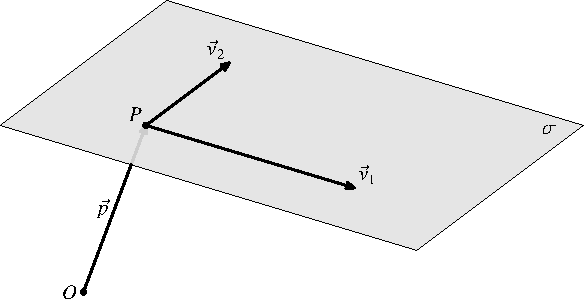
\includegraphics{images/v-8}
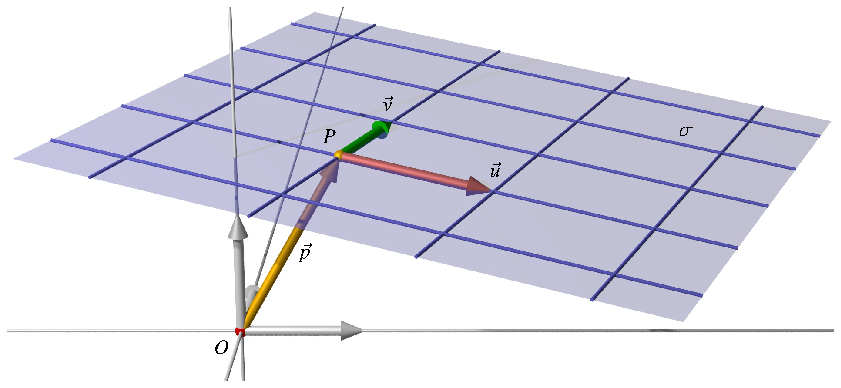
\includegraphics{3/images/ebene.pdf}
\end{center}
\caption{Parametrisierung einer Ebene mit Stüztvektor $\vec{p}$ und
Richtungsvektoren $\vec{u}$ und $\vec{v}$.
\label{image-parametrisierungebene}}
\end{figure}%
Ebenen zeichnen sich gegenüber Geraden dadurch aus, dass sich auf ihnen
ein Punkt nicht nur in einer Richtung, sondern unabhängig zwei Richtungen
bewegen kann.
Wir brauchen also einen zweiten Richtungsvektor und einen zweiten Parameter.
Die Punkte einer Ebene $\sigma$ werden also beschrieben durch
\[
\vec r=\vec p+t\vec v_1+s\vec v_2,
\]
(Abbildung~\ref{image-parametrisierungebene}).

\begin{beispiel}
Man finde die Parameterdarstellung der Ebene durch die Punkte
$A=(1,2,1)$,
$B=(3,4,-1)$ und
$C=(4,-1,0)$.

\smallskip

{\parindent 0pt Die} Vektoren $\vec u=\overrightarrow{AB}$ und
$\vec v=\overrightarrow{AC}$ können als Richtungsvektoren
verwendet werden, und ergeben als Parameterdarstellung:
\begin{equation}
\vec r=\begin{pmatrix}1\\2\\1 \end{pmatrix}
+
t\begin{pmatrix}2\\2\\-2\end{pmatrix}
+
s\begin{pmatrix}3\\-3\\-1\end{pmatrix}.
\label{beispielebene}
\end{equation}
\end{beispiel}

\subsection{Durchstosspunkt\label{subsection-durchstosspunkt}}
\index{Durchstosspunkt}
\begin{figure}
\begin{center}
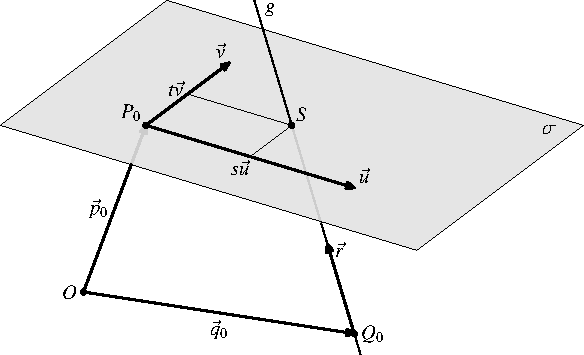
\includegraphics{images/v-9}
\end{center}
\caption{Durchstosspunkt $S$ der Geraden $g$ durch die Ebene
$\sigma$.\label{image-durchstosspunkt}}
\end{figure}
Im dreidimensionalen Raum
sind eine Gerade $g$ und eine Ebene $\sigma$ je in Parameterdarstellung gegeben, also
\begin{align*}
\sigma&=
\{
\vec p_0+s\vec u+t\vec v\;
|\;s, t\in\mathbb R\}
\\
g&=
\{
\vec q_0+l\vec r\;
|\;l\in\mathbb R
\}
\end{align*}
Es soll der Durchstosspunkt $S$ der Gerade durch die Ebene gefunden
werden (Abbildung~\ref{image-durchstosspunkt}).
Dazu müssen wir die Parameterwerte für $s$, $t$ und $l$ finden,
für die gilt
\begin{align*}
\vec p_0+s\vec u+t\vec v
&=
\vec q_0+l\vec r
\\
s\vec u+t\vec v-l\vec r&=\vec q_0+\vec p_0
\end{align*}
Dies ist eine Vektorgleichung mit den drei Unbekannten $s$, $t$ und $l$,
sie entspricht drei linearen Gleichungen für diese Unbekannten.

Im Allgemeinen wird dieses Gleichungssystem genau eine Lösung haben,
nämlich den Durchstosspunkt.
Ist die Gerade parallel zur Ebene, hat das Gleichungssystem jedoch keine
Lösung, es gibt also auch keinen Durchstosspunkt.
Liegt die Gerade dagegen in der Ebene, gibt es unendlich viele Lösungen.

In den singulären Fällen ist es offenbar möglich, die Richtung $\vec r$
der Gerade durch die beiden Vektoren $\vec u$ und $\vec v$ in der Ebene
auszudrücken, die drei Vektoren $\vec u$, $\vec v$ und $\vec r$ sind
linear abhängig.

\begin{beispiel}
Finde den Durchstosspunkt der Geraden
\[
\vec r=
\begin{pmatrix} 5\\8\\3 \end{pmatrix}
+
l\begin{pmatrix} 1\\0\\1 \end{pmatrix}
\]
durch die Ebene (\ref{beispielebene}).

\smallskip

{\parindent0pt Zusammen} mit der Gleichung (\ref{beispielebene}) bekommen wir die
Vektorgleichung
\[
\begin{pmatrix}1\\2\\1 \end{pmatrix}
+
t\begin{pmatrix}2\\2\\-2\end{pmatrix}
+
s\begin{pmatrix}3\\-3\\-1\end{pmatrix}
=
\begin{pmatrix} 5\\8\\3 \end{pmatrix}
+
l\begin{pmatrix} 1\\0\\1 \end{pmatrix}
\quad\Rightarrow\quad
t\begin{pmatrix}2\\2\\-2\end{pmatrix}
+
s\begin{pmatrix}3\\-3\\-1\end{pmatrix}
+
l\begin{pmatrix} -1\\0\\-1 \end{pmatrix}
=
\begin{pmatrix} 4\\6\\2 \end{pmatrix}
\]
Das Gleichungssystem kann mit dem Gauss-Algorithmus
gelöst werden
\begin{align*}
\begin{tabular}{|>{$}c<{$}>{$}c<{$}>{$}c<{$}|>{$}c<{$}|}
\hline
 2%
\begin{picture}(0,0)
\color{red}\put(-3,4){\circle{12}}
\end{picture}%
& 3&-1&4\\
 2&-3& 0&6\\
-2%
\begin{picture}(0,0)
\color{blue}\drawline(-15,-2)(-15,24)(2,24)(2,-2)
\end{picture}
&-1&-1&2\\
\hline
\end{tabular}
&
\rightarrow
\begin{tabular}{|>{$}c<{$}>{$}c<{$}>{$}c<{$}|>{$}c<{$}|}
\hline
 1& \frac32&-\frac12&2\\
 0&-6%
\begin{picture}(0,0)
\color{red}\put(-7,3){\circle{15}}
\end{picture}%
& 1&2\\
 0& 2&-2&6\\
\hline
\end{tabular}
\rightarrow
\begin{tabular}{|>{$}c<{$}>{$}c<{$}>{$}c<{$}|>{$}c<{$}|}
\hline
 1& \frac32&-\frac12&2\\
 0& 1&-\frac16&-\frac13\\
 0& 0&-\frac53%
\begin{picture}(0,0)
\color{red}\put(-7,3){\circle{16}}
\end{picture}%
&\frac{20}3\\
\hline
\end{tabular}
\\
&
\rightarrow
\begin{tabular}{|>{$}c<{$}>{$}c<{$}>{$}c<{$}|>{$}c<{$}|}
\hline
 1& \frac32&-\frac12&2\\
 0& 1&-\frac16%
\begin{picture}(0,0)
\color{blue}\drawline(-15,24)(-15,-5)(2,-5)(2,24)
\end{picture}
&-\frac13\\
 0& 0& 1&-4\\
\hline
\end{tabular}
\rightarrow
\begin{tabular}{|>{$}c<{$}>{$}c<{$}>{$}c<{$}|>{$}c<{$}|}
\hline
 1& \frac32%
\begin{picture}(0,0)
\color{blue}\drawline(-8,10)(-8,-5)(2,-5)(2,10)
\end{picture}%
& 0&0\\
 0& 1& 0&-1\\
 0& 0& 1&-4\\
\hline
\end{tabular}
\\
&
\rightarrow
\begin{tabular}{|>{$}c<{$}>{$}c<{$}>{$}c<{$}|>{$}c<{$}|}
\hline
 1& 0& 0&\frac32\\
 0& 1& 0&-1\\
 0& 0& 1&-4\\
\hline
\end{tabular}
\end{align*}
Da $l=-4$ kann man jetzt den Durchstosspunkt berechnen, er ist $S=(1,8,-1)$.
\end{beispiel}

\subsection{Schnittgerade}
\index{Schnittgerade zweier Ebenen}
\begin{figure}
\begin{center}
%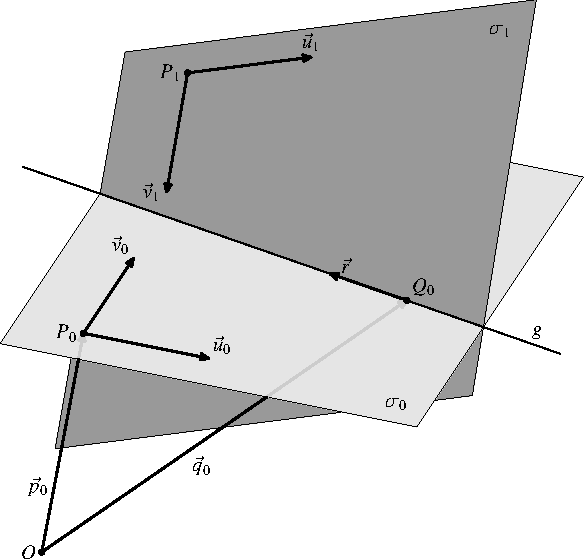
\includegraphics{images/v-10}
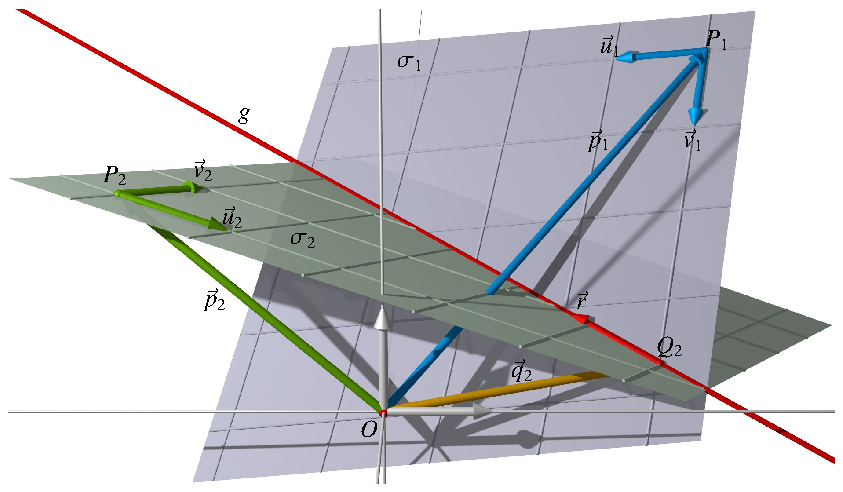
\includegraphics{3/images/schnittgerade.pdf}
\end{center}
\caption{Schnittgerade $g$ (rot) zweier Ebenen $\sigma_0$ (grün)
und $\sigma_1$ (blau).
\label{image-schnittgerade}}
\end{figure}
Im dreidimensionalen Raum sind zwei Ebenen
\begin{align*}
\sigma_0&=
\{\vec p_0+s_0\vec u_0+t_0\vec v_0\;|\;s_0, t_0\in\mathbb R\}
\\
\sigma_1&=
\{\vec p_1+s_1\vec u_1+t_1\vec v_1\;|\;s_1, t_1\in\mathbb R\}
\end{align*}
gegeben, gesucht ist deren Schnittgerade $g$
(Abbildung~\ref{image-schnittgerade}).
Diese besteht offenbar aus den Punkten, die sich für geeignete Parameterwerte
$s_0,t_0,s_1,t_1$ mit der Eigenschaft
\begin{align*}
p_0+s_0\vec u_0+t_0\vec v_0
&=
p_1+s_1\vec u_1+t_1\vec v_1
\\
s_0\vec u_0+t_0\vec v_0
-s_1\vec u_1-t_1\vec v_1
&=
-p_0+
p_1
\end{align*}
finden lassen.
Dies ist ein Gleichungssystem mit drei Gleichungen für
vier Unbekannte, im Allgemeinen wird sich also eine der Unbekannten
nicht bestimmen lassen, sondern die anderen Unbekannten werden sich
durch die vierte ausdrücken lassen.
Die Punkte der Schnittmenge sind also von der Form
\[
p_1+s_1(t_1)\vec u_1+t_1\vec v_1,
\]
wobei von der Form $s_1(t_1)=a+bt_1$ sein muss.
Setzt man dies ein, ergibt sich wieder eine Geradengleichung:
\[
p_1+s_1(t_1)\vec u_1+t_1\vec v_1
=
p_1+(a+bt_1)\vec u_1+t_1\vec v_1
=
(p_1+a\vec u_1)+t_1(b\vec u_1+v_1),
\]
eine Geradengleichung mit Richtungsvektor $\vec r = (b\vec u_1+v_1)$ und
Ausgangspunkt $\vec q_0=p_1+a\vec u_1$, also mit der Parametrisierung
\[
g=\{\vec q_0+t\vec r\;|\;t\in\mathbb R\}.
\]

\begin{beispiel}
Man finde die Schnittgerade der beiden Ebenen mit Parameterdarstellung
\[
\sigma_0:
\vec p_0+s_0\vec u_0+t_0\vec v_0
=\begin{pmatrix}5\\8\\6\end{pmatrix}
+s_0\begin{pmatrix}4\\6\\7\end{pmatrix}
+t_0\begin{pmatrix}2\\5\\6\end{pmatrix}
,
\qquad
\sigma_1:
\vec p_1+s_1\vec u_1+t_0\vec v_1
=\begin{pmatrix}5\\4\\4\end{pmatrix}
+s_1\begin{pmatrix}6\\6\\7\end{pmatrix}
+t_1\begin{pmatrix}5\\4\\4\end{pmatrix}
\]

\smallskip

{\parindent 0pt Wir setzen die beiden Parametrisierungen gleich und
erhalten}
\[
\begin{pmatrix}5\\8\\6\end{pmatrix}
+s_0\begin{pmatrix}4\\6\\7\end{pmatrix}
+t_0\begin{pmatrix}2\\5\\6\end{pmatrix}
=\begin{pmatrix}5\\4\\4\end{pmatrix}
+s_1\begin{pmatrix}6\\6\\7\end{pmatrix}
+t_1\begin{pmatrix}5\\4\\4\end{pmatrix}
\]
oder
\[
s_0\begin{pmatrix}4\\6\\7\end{pmatrix}
+t_0\begin{pmatrix}2\\5\\6\end{pmatrix}
-s_1\begin{pmatrix}6\\6\\7\end{pmatrix}
-t_1\begin{pmatrix}5\\4\\4\end{pmatrix}
=
\begin{pmatrix}0\\-4\\-2\end{pmatrix}
\]
Der Gauss-Algorithmus liefert für die Lösung das Tableau
\[
\begin{tabular}{|>{$}c<{$}>{$}c<{$}>{$}c<{$}>{$}c<{$}|>{$}c<{$}|}
\hline
4&2&-6&-5& 0\\
6&5&-6&-4&-4\\
7&6&-7&-4&-2\\
\hline
\end{tabular}
\rightarrow
\begin{tabular}{|>{$}c<{$}>{$}c<{$}>{$}c<{$}>{$}c<{$}|>{$}c<{$}|}
\hline
    1&   0&   0& -\frac{11}2& -26\\
    0&   1&   0&   4&  16\\
    0&   0&   1&  -\frac32& -12\\
\hline
\end{tabular}
\]
Die Variable $t_1$ ist frei wählbar, daraus lassen sich die anderen
Variablen bestimmen:
\[
\begin{linsys}{3}
s_0&=&-26&+&\frac{11}2t_1\\
t_0&=&16&-&4t_1\\
s_1&=&-12&+&\frac32t_1\\
\end{linsys}
\]
Setzt man dies in die ursprünglichen Ebenengleichungen ein, entsteht
die Parameterdarstellung der Schnittgeraden:
\begin{align*}
\begin{pmatrix}x\\y\\z\end{pmatrix}
&=
\begin{pmatrix}5\\8\\6\end{pmatrix}
+\biggl(-26+\frac{11}2t_1\biggr)\begin{pmatrix}4\\6\\7\end{pmatrix}
+(16-4t_1)\begin{pmatrix}2\\5\\6\end{pmatrix}
=
\begin{pmatrix}-67\\-68\\-80\end{pmatrix}
+t_1
\begin{pmatrix}14\\13\\\frac{29}2\end{pmatrix},\quad\text{oder}
\\
\begin{pmatrix}x\\y\\z\end{pmatrix}
&=
\begin{pmatrix}5\\4\\4\end{pmatrix}
+\biggl(-12+\frac32t_1\biggr)\begin{pmatrix}6\\6\\7\end{pmatrix}
+t_1\begin{pmatrix}5\\4\\4\end{pmatrix}
=
\begin{pmatrix}-67\\-68\\-80\end{pmatrix}
+t_1
\begin{pmatrix}14\\13\\\frac{29}2\end{pmatrix}
\end{align*}
Natürlich muss man in beiden Fällen die gleiche Gerade bekommen,
dies ist eine hübsche Kontrolle für die Richtigkeit des Resultates.
\end{beispiel}

\subsection{Vereinheitlichtes Lösungsverfahren\label{section-vereinheitlichtes-verfahren}}
Alle in den bisherigen Abschnitten vorgestellten Lösungsverfahren
laufen darauf hinaus, dass man für die Parameter der Parameterdarstellungen
Gleichungen dadurch aufstellt, dass man wo nötig Gleichungen herstellt.
Dies ist aber eigentlich ein unnötiger Schritt, den man auch dem
Gauss-Algorithmus überlassen könnte.

Traditionell wird das so gemacht, weil früher eine grosse Angst
davor bestand, auf grosse Gleichungssysteme zu stossen, deren Lösung
mühsam ist.
Diese Angst ist heute mit modernen Taschenrechnern und
Computer nicht mehr gerechtfertigt.

\subsubsection{Durchstosspunkt}
Um den Durchstosspunkt wie in \ref{subsection-durchstosspunkt} zu finden,
gehen wir wieder von den Parameterdarstellungen aus, schreiben jetzt
aber den gesuchten gemeinsamen Ortsvektor des Punktes
$({\color{red}x}, {\color{red}y}, {\color{red}z})$ explizit hin:
\[
\begin{pmatrix}
\color{red}x\\
\color{red}y\\
\color{red}z\\
\end{pmatrix}
=
\begin{pmatrix}1\\2\\1 \end{pmatrix}
+
{\color{red}t}\begin{pmatrix}2\\2\\-2\end{pmatrix}
+
{\color{red}s}\begin{pmatrix}3\\-3\\-1\end{pmatrix}
,\qquad
\begin{pmatrix}
\color{red}x\\
\color{red}y\\
\color{red}z\\
\end{pmatrix}
=
\begin{pmatrix} 5\\8\\3 \end{pmatrix}
+
{\color{red}l}\begin{pmatrix} 1\\0\\1 \end{pmatrix}
\]
Darin haben wir alle unbekannten Grössen {\color{red}rot} markiert.
Wir haben jetzt sechs Gleichungen mit sechs Unbekannten.
Der Gauss-Algorithmus liefert direkt die Lösung, sofern es eine gibt,
ohne dass man wie in Abschnitt \ref{subsection-durchstosspunkt}
die gefundenen Parameterwerte nochmals einsetzen müsste:
\[
\begin{tabular}{|>{$}c<{$}>{$}c<{$}>{$}c<{$}>{$}c<{$}>{$}c<{$}>{$}c<{$}|>{$}c<{$}|}
\hline
{\color{red}x}&
{\color{red}y}&
{\color{red}z}&
{\color{red}t}&
{\color{red}s}&
{\color{red}l}&\\
\hline
1&0&0&-2&-3& 0&1\\
0&1&0&-2& 3& 0&2\\
0&0&1& 2& 1& 0&1\\
1&0&0& 0& 0&-1&5\\
0&1&0& 0& 0& 0&8\\
0&0&1& 0& 0&-1&3\\
\hline
\end{tabular}
\rightarrow
\begin{tabular}{|>{$}c<{$}>{$}c<{$}>{$}c<{$}>{$}c<{$}>{$}c<{$}>{$}c<{$}|>{$}c<{$}|}
\hline
{\color{red}x}&
{\color{red}y}&
{\color{red}z}&
{\color{red}t}&
{\color{red}s}&
{\color{red}l}&\\
\hline
1&0&0&0&0&0&1\\
0&1&0&0&0&0&8\\
0&0&1&0&0&0&-1\\
0&0&0&1&0&0&1.5\\
0&0&0&0&1&0&-1\\
0&0&0&0&0&1&-4\\
\hline
\end{tabular}
\]
Daraus liest man einerseits den Durchstosspunkt $(1,8,-1)$ ab, andererseits
findet man die Parameterwerte, für die dieser Durchstosspunkt erreicht wird.

\subsubsection{Schnittgerade}
Die Schnittgerade der zwei Ebenen kann wie folgt gefunden werden.
Zunächst beschreiben wir mit der Parameterdarstellung, wie der
Ortsvektor eines beliebigen Punktes $(x,y,z)$ der Ebenen entsteht:
\[
\begin{pmatrix}
\color{red}x\\
\color{red}y\\
\color{red}z\\
\end{pmatrix}
=
\begin{pmatrix}5\\8\\6\end{pmatrix}
+{\color{red}s_0}\begin{pmatrix}4\\6\\7\end{pmatrix}
+{\color{red}t_0}\begin{pmatrix}2\\5\\6\end{pmatrix}
,\qquad
\begin{pmatrix}
\color{red}x\\
\color{red}y\\
\color{red}z\\
\end{pmatrix}
=
\begin{pmatrix}5\\4\\4\end{pmatrix}
+{\color{red}s_1}\begin{pmatrix}6\\6\\7\end{pmatrix}
+{\color{red}t_1}\begin{pmatrix}5\\4\\4\end{pmatrix}
\]
Hier hat man plötzlich 6 Gleichungen für 7 Unbekannte.
Wir erwarten also eine frei wählbare Variable, die dann als Parameter
für die Schnittgerade dienen kann.
Das Gausstableau ist
\[
\begin{tabular}{|>{$}c<{$}>{$}c<{$}>{$}c<{$}>{$}c<{$}>{$}c<{$}>{$}c<{$}>{$}c<{$}|>{$}c<{$}|}
\hline
{\color{red}x}&
{\color{red}y}&
{\color{red}z}&
{\color{red}s_0}&
{\color{red}t_0}&
{\color{red}s_1}&
{\color{red}t_1}&\\
\hline
1&0&0&-4&-2& 0& 0&5\\
0&1&0&-6&-5& 0& 0&8\\
0&0&1&-7&-6& 0& 0&6\\
1&0&0& 0& 0&-6&-5&5\\
0&1&0& 0& 0&-6&-4&4\\
0&0&1& 0& 0&-7&-4&4\\
\hline
\end{tabular}
\rightarrow
\begin{tabular}{|>{$}c<{$}>{$}c<{$}>{$}c<{$}>{$}c<{$}>{$}c<{$}>{$}c<{$}>{$}c<{$}|>{$}c<{$}|}
\hline
{\color{red}x}&
{\color{red}y}&
{\color{red}z}&
{\color{red}s_0}&
{\color{red}t_0}&
{\color{red}s_1}&
{\color{red}t_1}&\\
\hline
1&0&0&0&0&0&         - 14\phantom{.0}&-67\\
0&1&0&0&0&0&         - 13\phantom{.0}&-68\\
0&0&1&0&0&0&         - 14.5          &-80\\
0&0&0&1&0&0&-\phantom{0}5.5          &-26\\
0&0&0&0&1&0&\phantom{-0}4\phantom{.0}&\phantom{-}16\\
0&0&0&0&0&1&-\phantom{0}1.5          &-12\\
\hline
\end{tabular}
\]
Daraus liest man ab, dass es unendlich viele Punkte gibt, die auf beiden
Ebenen liegen, und dass $t_1$ als Parameter für die Geradengleichung
dienen kann.
Ausserdem kann man die Parameterdarstellung der Gerade ablesen:
\[
\begin{pmatrix}-67\\-68\\-80\end{pmatrix}
+t_1
\begin{pmatrix}14\\13\\14.5\end{pmatrix}.
\]





%
% vektorraum.tex
%
% (c) 2017 Prof Dr Andreas Müller, Hochschule Rapperswil
%
\chapter{Vektorraum}
Wenn angehende Ingenieure zum ersten Mal mit linearer Algebra in
Kontakt kommen, arbeiten sie meistens mit Spaltenvektoren von
reellen Zahlen.
Diese Vektoren können mit reellen Zahlen multipliziert werden,
Vektoren können addiert und subtrahiert werden.
Später kommen Matrizen hinzu, welche oft als eine rein formale
Erweiterung der Vektoren betrachtet werden können, als ``dicke''
Vektoren, für die es eine zusätzliche Verknüpfung mit Vektoren
gibt.
Entsprechend liegt das Schwergewicht oft auf Anwendungen in der
Vektorgeometrie.

Dabei gerät oft in Vergessenheit, dass auch ein viel grösseres
Anwendungsgebiet zum Beispiel in der Analysis oder der Kryptographie
haben.
Auch Funktionen können addiert, subtrahiert und mit reellen Zahlen
multipliziert werden.
Auch für Funktionen kann man ein Skalarprodukt definieren, und
damit die geometrisch Idee der orthonormierten Basis und der
einfachen Zerlegung bezüglich einer Basis für Funktionen nutzen,
dies ist die geometrische Betrachtungsweise der Fourier-Theorie.

Damit man die Erkenntnisse der linearen Algebra in dieser Form
nutzen kann, muss man sich erst von der Fixierung auf Spaltenvektoren
lösen.
Man muss also die grundlegende Theorie zuerst so abstrakt formulieren,
dass sie tatsächlich auf die genannten Situationen angewendet werden 
kann.


%
% skalare.tex
%
% (c) 2017 Prof Dr Andreas Müller, Hochschule Rapperswil
%
\section{Skalare -- Körper}
In der elementaren lineare Algebra können Vektoren mit reellen
Zahlen multipliziert werden, Zahlen können mit Zahlen multiplizert
werden, Vektoren mit Vektoren, aber es gibt keine Multiplikation
von Vektoren.
Ausserdem kann man natürlich durch beliebige reelle Zahlen teilen,
eine wesentliche Voraussetzung für die Lösung von linearen Gleichungssysteme.
Die lineare Algebra unterscheidet also Objekte, die nicht miteinander
multipliziert werden können und solche, für die alle arithmetischen
Operationen möglich sind.

Die reellen Zahlen haben aber noch viel mehr Struktur, welche in
der linearen Algebra nicht benötigt werden.
Zum Beispiel können positive und negative reelle Zahlen unterschieden
werden, eine Eigenschaft, die für die Lösung linearer Gleichungssyteme
irrelevant zu sein scheint.
Jede Cauchy-Folge reeller Zahlen hat einen Grenzwert, doch das Konzept
des Grenzwertes spielt in der elementaren linearen Algebra ebenfalls
keine Rolle.

Ziel dieses Kapitel ist daher, die tatsächlich nötigen, minimalen
Anforderungen an die Skalare in der linearen Algebra zu formulieren.
Dabei wird die Struktur des Zahlkörpers in den Vordergrund gerückt
und weitere Beispiele von Zahlkörpern werden besprochen.
Der Fall der endlichen Körper wird im Kapitel~\ref{chapter:endlichekoerper}
im Detail untersucht.

\subsection{Skalare}
Welche Operation nötig sind, um lineare Gleichungssysteme zu lösen
verraten schon das einfachsten lineare Gleichungsysteme.
Aus dem $1\times 1$-Gleichungssystem 
\[
ax=b\qquad\Rightarrow\qquad x=\frac{b}{a}
\]
folgt, dass man durch beliebige von $0$ verschiedene Elemente dividieren
können muss.
Das Gleichungssystem
\[
\left.
\begin{linsys}{3}
ax&+&by&=&c\\
  & &dy&=&e
\end{linsys},
\right\}
\qquad\Rightarrow\qquad
y=\frac{e}{d},\quad
x=\frac1{a}\biggl(c-b\frac{e}{d}\biggr)
\]
kann nur gelöst werden, wenn auch die Subtraktion zur Verfügung steht.
Eine im Sinne des Ziels der Lösung linearer Gleichungen sinnvolle 
Theorie kann also nur aufgebaut werden, wenn alle arithmetischen
Grundoperationen zur Verfügung stehen.

Mehr als die arithmetischen Grundoperationen ist erst dann nötig, 
wenn man Eigenwerte bestimmen will. 
Dann müssen zum Beispiel Nullstellen des charakteristischen Polynoms
bestimmt werden.
Doch einfache Bespiele zeigen, dass dies nicht einmal in den reellen
Zahlen immer möglich ist.
Das Ziel muss daher sein, Zahlenmengen zu charakterisieren, die die
Rolle der Skalare in der linearen Algebra übernehmen können.
Eine solche Menge muss die Lösung beliebiger lineare Gleichungssysteme
ermöglichen, wir verlangen aber nicht, dass auch beliebige Eigenwertprobleme
gelöst werden können.

\subsection{Körper}
Die folgende Definition beschreibt eine Zahlenmenge, in der alle
Grundoperationen zur Verfügung stehen, eine solche Menge heisst
ein {\em Körper}.
\index{Körper}%

\begin{definition}
Sei $K$ eine Menge mit zwei Operationen, der Addition, geschrieben $+$,
und der Multiplikation, geschrieben $\cdot$, die die folgenden
Eigenschaften hat:
\begin{compactenum}
\item Die Addition ist assoziativ und kommutativ.
\item Es gibt ein neutrales Element $0\in K$ für die Addition,
d.~h.~$a+0=a$ für alle $a\in K$.a
\item Jede Gleichung $x+a=b$ mit $a,b\in K$ kann eindeutig nach $x$ aufgelöst
werden.
\item Die Multiplikation ist assoziativ und kommutativ.
\item Es gibt ein neutrales Element $1$ für die Multiplikation,
d.~h.~$1\cdot a=a$ für alle $a\in K$.
\item Jede Gleichung $ax=b$ mit $a,b\in K$ und $a\ne 0$ kann eindeutig 
nach $x$ aufgelöst werden, die Lösung wird $x=b/a=ba^{-1}$ geschrieben.
\item Für beliebige $a,b,c\in K$ gilt
$a(b+c)=ab+ac$.
\end{compactenum}
$K$ heisst ein {\em Körper}.
\end{definition}

Die Forderung nach Assoziativität stellt sicher, dass Summen oder
Produkte mit mehr als zwei Summanden bzw.~Faktoren in beliebiger
Reihenfolge berechnet werden können.

Die Forderung nach Kommutativität sieht im Moment vor allem nach
Bequemlichkeit aus.
Eine genauere Analyse des Gauss-Algorithmus zeigt jedoch, dass er 
nur für kommutative Skalare funktioniert.

Die Bedingung 3 definiert die Subtraktion während Bedingung 6
besagt, dass man auf eindeutige Art durch von $0$ verschiedene
Zahlen teilen kann.

Die Bedingung~7, das Distributivgesetz, stellt sicher,
dass die algebraischen Operationen
sich so verhalten, wie man es sich aus der Schule kennt.
Zum Beispiel kann die Gleichug $ax+b=c$ auf zwei Arten gelöst werden
\begin{align*}
\xymatrix{
\txt{}	&{ay+b=c}\ar[dr]\ar[dl]
\\
ay=c-b \ar[d]	&\txt{}	&y+ba^{-1}=ca^{-1}\ar[d]
\\
y=(c-b)a^{-1}&\txt{}&	y=ca^{-1}-ba^{-1}
}
\end{align*}
Auf dem linken Ast wir erst die Konstante $b$ auf die rechte Seite
gebracht, auf dem rechten wird erst durch $a$ dividiert.
Natürlich sollten beide Lösungen übereinstimmen, dies ist nur möglich,
wenn das Distributivgesetz gilt.

\subsection{Beispiele}
Die reellen Zahlen bilden ganz offensichtlich einen Körper.
Andererseits bilden die ganzen Zahlen ganz bestimmt keinen Körper,
denn die Gleichung $2x=1$ hat keine ganzzahlige Lösung, im Widerspruch
zu Eigenschaft~6 eines Körpers.
Auch die natürlichen Zahlen bilden keinen Körper, denn die Gleichung
$x+1=0$ hat keine Lösung in $\mathbb N$, im Widerspruch zur Eigenschaft~3
eines Körpers.
In diesem Kapitel sollen daher ein paar Beispiele von Köpern
zusammengestellt werden.

\subsubsection{Rationale Zahlen}
Die rationalen Zahlen $\mathbb Q$ erweitern die ganzen Zahlen $\mathbb Z$
so, dass beliebige Divisionen durchführen kann.
Die rationalen Zahlen bilden den kleinsten Körper, der die ganzen
Zahlen enthält.
Die ganze lineare Algebra liesse sich also auch ausschliesslich in
den rationalen Zahlen entwickeln.

\subsubsection{Quotientenkörper eines Ringes}
Die rationalen Zahlen enstanden dadurch, dass aus ganzen Zahlen $\mathbb Z$
Brüche konstruiert wurden.
Wenn wir die Elemente der Menge
\[
\{ (z,n)\,| z,n\in\mathbb Z\wedge n\ne 0\}
\]
als Brüche betrachten wollen, dann müssen wir zwei Brüche
$(z_1,n_1)$ und $(z_2,n_2)$ als gleich betrachten, wenn sie
übereinstimmen, sobald man sie gleichnamig gemacht hat.
Multipliziert man $(z_1,n_1)$ mit $n_2$ und $(z_2,n_2)$ mit $n_1$, dann
beschreiben die erweiterten Brüche
$(z_1n_2,n_1n_2)$ und $(z_2n_1,n_1n_2)$ die gleiche Zahl, wenn
$z_1n_2=z_2n_1$.
Eine rationale Zahl $q=z/n$ kann also betrachtet werden als die
Teilmenge
\[
q
=
M(q)
=
\{(z',n')\,|\, z',n'\in\mathbb Z\wedge n'\ne 0 \wedge zn'=z'n\}
\subset
\{(z',n')\,|\, z',n'\in\mathbb Z\wedge n'\ne 0\}.
\]
Die Menge der $M(q)$ kann betrachtet werden als die Menge der rationalen
Zahlen.

Diese Konstruktion kann verallgemeinert werden, wie wir an einem
Beispiel illustrieren wollen.
Sei $R=\mathbb R[X]$ die Menge der Polynome in der Variablen $X$
mit reellen Koeffizienten.
Die Axiome eines Körpers sind für $R$ nicht alle erfüllt.
Bedingung~6 ist nicht erfüllt, da man im Allgemeinen nicht durch Polynome
dividieren kann.

Motiviert durch die Konstruktion der Brüche kann man jedoch die Menge
der Brüche von Polynomen konstruieren.
Dazu betrachtet man zunächst die Menge
\[
\{ (p,q)\,|\, p,q\in \mathbb R[X]\wedge q\ne 0\}
\]
von Paaren von Polynomen.
Dann bildet man für ein vorgegebenens Paar von Polynomen $r=(p,q)$ die
Teilmenge
\[
M(r)
=
\{ (p',q')\,|\, p',q'\in \mathbb R[X]\wedge q'\ne 0\wedge pq'=p'q\}.
\]
Die Menge $M(r)$ besteht aus allen Polynombrüchen, die nach 
Gleichnamigmachen mit $q$ übereinstimmen.
Wir nennen die Menge 
\[
\mathbb R(X)
=
\{ M(r)\, |\, r=(p,q)\wedge p,q\in\mathbb R[X]\wedge q\ne 0\}
\]
die Menge der rationalen Funktionen in der Variablen $X$, sie ist
ein Körper.
Wir verwenden im Folgenden wieder die üblichere Schreibweise $p(X)/q(X)$
für $r\in\mathbb R(X)$.

Die Konstruktion der Brüche funktioniert, solange die Operation des
Gleichnamigmachens wohldefiniert ist.
Dazu ist zunächst notwendig, dass bleibige Multiplikationen ausführbar
sind.
Eine Menge $R$, die alle Axiome eines Körpers ausser 5 und 6 erfüllt,
heisst ein kommutativer Ring.

Dann ist notwendig, dass die Multiplikation der Nenner nie auf $0$ führt.
Man nennt $R$ einen {\em Integritätsbereich},
wenn $n_1n_2\ne 0$ für beliebige $n_1,n_2\ne 0$.
\index{Integritätsbereich}%
Die Konstruktion der Brüche ist also möglich für beliebige
Integritätsbereiche.

\subsubsection{Komplexe Zahlen}
Die Menge $\mathbb C$ der komplexen Zahlen entstehen aus der Menge $\mathbb R$
der reellen Zahlen dadurch, dass man ein neues Element $i$ mit der Eigenschaft
$i^2=-1$ hinzufügt, dabei aber alle anderen Rechenregeln beibehält.
Da das Quadrat von $i$ wieder eine reelle Zahl ist, kann man jede beliebige
komplexe Zahl in der Form $a+bi$ schreiben.
Es stellt sich heraus, dass man in der Menge der komlexen Zahlen beliebig
divideren kann:
\[
\frac{a+bi}{c+di}
=
\frac{a+bi}{c+di}
\cdot
\frac{c-di}{c-di}
=
\frac{ac-bd + i(ad+bc)}{c^2 + d^2},
\]
natürlich nur, wenn $c^2+d^2\ne 0$ oder $c+di\ne 0$.
Die Menge $\mathbb C$ ist also ein Körper.

Die besondere Bedeutung der komplexen Zahlen für die lineare Algebra ist, 
dass darin nicht nur Gleichungssyteme gelöst werden können.
In $\mathbb C$ kann auch jede Polynomgleichung gelöst werden, so dass
sich das Eigenwertproblem immer lösen lässt.

\subsubsection{Endliche Körper}
In der Menge $\mathbb F_p=\mathbb F_5$ der Reste bezüglich der Primzahl
$p=5$ sind die Addition und die Multiplikation wohldefiniert.
Die Additions- und Multiplikationstabellen sind
\[
\begin{tabular}{|c|ccccc|}
\hline
$+$&0&1&2&3&4\\
\hline
0&0&1&2&3&4\\
1&1&2&3&4&0\\
2&2&3&4&0&1\\
3&3&4&0&1&2\\
4&4&0&1&2&3\\
\hline
\end{tabular}
\qquad
\begin{tabular}{|c|ccccc|}
\hline
$\cdot$&0&1&2&3&4\\
\hline
0&0&0&0&0&0\\
1&0&1&2&3&4\\
2&0&2&4&1&3\\
3&0&3&1&4&2\\
4&0&4&3&2&1\\
\hline
\end{tabular}
\]
Da in jeder Zeile jede Zahl genau einmal vorkommt (ausser in den ersten
Zeilen und Spalte in der Multiplikationstabelle) kann man schliessen, dass
die Menge $\mathbb F_5$ die Bedingungen 3 und 6 eines Körpers erfüllt.
Somit ist $\mathbb F_5$ ein Körper.
Es gilt sogar allgemein für jede beliebige Primzahl, dass die Menge
$\mathbb F_p$ ein Körper ist.
Im Gegensatz zu den bereits untersuchten Körpern ist $\mathbb F_p$ endlich.
Die lineare Algebra in endlichen Körpern wird in
Kapitel~\ref{chapter:endlichekoerper} genauer untersucht.

Allerdings lassen sich nicht alle Polynomgleichungen mit Koeffizienten
in $\mathbb F_5$ lösen.
Die Gleichung
\[
x^2-2=0
\]
hat keine Lösung in $\mathbb F_5$, wie man durch Inspektion der
Multiplikationstabelle einsehen kann.


\subsection{Körpererweiterungen}
Die Körper der rationalen Zahlen und der reellen Zahlen sind insofern
nicht optimal für die lineare Algebra, dass sich das Eigenwertproblem
nicht immer lösen lässt.
Dabei wäre es nur nötig, dass der Körper die Nullstellen des
charakteristischen Polynoms enthält. 
Die Matrix
\[
J=\begin{pmatrix}0&-1\\1&0\end{pmatrix}
\]
hat das charakteristische Polynom
\[
\varphi_{J}(\lambda)
=
\left|\begin{matrix}-\lambda&-1\\1&-\lambda\end{matrix}\right|
=
\lambda^2+1 = 0
\qquad\Rightarrow\qquad
\lambda=\pm i.
\]
Die Eigenwerte von $J$ sind also nicht im Körper enthalten,
und damit können auch die Eigenvektoren nicht reell sein.

Betrachtet man $J$ dagegen als komplexe Matrix, lassen sich sofort
Eigenvektoren für die Eigenwerte $\pm i$ angeben.
Dazu verwendet man den Gauss-Algorithmus auf die Matrix $J\pm iI$ an:
\[
\begin{aligned}
\begin{tabular}{|>{$}c<{$}>{$}c<{$}|>{$}c<{$}|}
\hline
         - i&-1&0\\
\phantom{-}1&-i&0\\
\hline
\end{tabular}
&\rightarrow
\begin{tabular}{|>{$}c<{$}>{$}c<{$}|>{$}c<{$}|}
\hline
 1&         - i&0\\
 0&\phantom{-}0&0\\
\hline
\end{tabular}
&&\Rightarrow
&
v_+&=\begin{pmatrix}i\\1\end{pmatrix},
&
Jv_+&=\begin{pmatrix}-1\\i\end{pmatrix}
=
i\begin{pmatrix}i\\1\end{pmatrix}
=
iv_+,
\\
\begin{tabular}{|>{$}c<{$}>{$}c<{$}|>{$}c<{$}|}
\hline
\phantom{-}i&         - 1&0\\
\phantom{-}1&\phantom{-}i&0\\
\hline
\end{tabular}
&\rightarrow
\begin{tabular}{|>{$}c<{$}>{$}c<{$}|>{$}c<{$}|}
\hline
 1&\phantom{-}i&0\\
 0&\phantom{-}0&0\\
\hline
\end{tabular}
&&\Rightarrow
&
v_-&=\begin{pmatrix}-i\\1\end{pmatrix},
&
Jv_-&=\begin{pmatrix}1\\i\end{pmatrix}
=
-i\begin{pmatrix}-i\\1\end{pmatrix}
=
-iv_-.
\end{aligned}
\]
Das Eigenwertproblem ist also vollständig lösbar geworden, indem
man dem ursprünglichen Körper genau die fehlenden Elemente, in diesem
Fall $i$ und $-i$ hinzugefügt hat, und wieder dafür gesorgt hat, dass
man einen Körper hat.
So ist der Körper $\mathbb C$ entstanden.

Man kann die Matrix $J$ aber auch als rationale Matrix betrachten.
Nach den eben gezeigten Lösung des Eigenwertproblems müsste es also
reichen, den rationalen Zahlen $\mathbb Q$ nur die imaginäre Einheit $i$
hinzuzufügen.
So erhält man eine Teilmenge
\[
\mathbb Q(i) = \{a+bi\,|\, a,b\in\mathbb Q\} \subset \mathbb C
\]
der komplexen Zahlen mit rationalen Komponenten.
Damit haben wir einen neuen Körper zwischen $\mathbb Q$ und $\mathbb C$
gefunden, der gross genug ist, das Eigenwertproblem für $J$ zu lösen.

\subsubsection{Körpererweiterung von $\mathbb Q$}
Wir versuchen dasselbe Vorgehen für das Eigenwertproblem für die Matrix
\[
A
=
\begin{pmatrix}
3&1\\
1&1
\end{pmatrix}.
\]
Die rationale Matrix $A$ hat das charakteristische Polynom
\[
\chi_{A}(\lambda)
=
\left|\begin{matrix}3-\lambda&1\\1&1-\lambda\end{matrix}\right|
=
(3-\lambda)(1-\lambda)-1
=
\lambda^2-4\lambda+2
\]
mit den Nullstellen
\[
\lambda_{\pm} = 2\pm\sqrt{4-2}=2\pm\sqrt{2} \not\in \mathbb Q.
\]
Zwischen den Zahlen $\lambda_+$ und $\lambda_-$ besehen die Beziehungen
\begin{align*}
\lambda_+ + \lambda_-=4
\quad&\Rightarrow\quad \lambda_-=4-\lambda_+
\\
\lambda_+\lambda_- = 2
\quad&\Rightarrow\quad \lambda_-=\frac{2}{\lambda_+}.
\end{align*}
Fügen wir die Zahl $\lambda_+$ den rationalen Zahlen hinzu sowie alle
Zahlen, die sich mit Hilfe der Körperoperationen daraus bilden lassen,
dann erhalten wir einen Körper, den wir
\[
\mathbb Q(2+\sqrt{2})
=
\{ a+b(2+\sqrt{2})\,|\, a,b\in\mathbb Q\}
=
\{ a + b\sqrt{2}\,|\,a,b\in\mathbb Q\}
=
\mathbb Q(\!\sqrt{2})
\]
bezeichnen.
In diesem Körper können wir jetzt das Eigenwertproblem für die Matrix $A$
lösen:
\[
\begin{aligned}
\begin{tabular}{|>{$}c<{$}>{$}c<{$}|}
\hline
3-\lambda_+&1          \\
1          &1-\lambda_+\\
\hline
\end{tabular}
&=
\begin{tabular}{|>{$}c<{$}>{$}c<{$}|}
\hline
1-\sqrt{2}& 1         \\
1         &-1-\sqrt{2}\\
\hline
\end{tabular}
\rightarrow
\begin{tabular}{|>{$}c<{$}>{$}c<{$}|}
\hline
1&-1-\sqrt{2}\\
0&0          \\
\hline
\end{tabular}
&&\Rightarrow&v_+&=\begin{pmatrix}1+\sqrt{2}\\1\end{pmatrix}
\\
\begin{tabular}{|>{$}c<{$}>{$}c<{$}|}
\hline
3-\lambda_-&1          \\
1          &1-\lambda_-\\
\hline
\end{tabular}
&=
\begin{tabular}{|>{$}c<{$}>{$}c<{$}|}
\hline
1+\sqrt{2}& 1         \\
1         &-1+\sqrt{2}\\
\hline
\end{tabular}
\rightarrow
\begin{tabular}{|>{$}c<{$}>{$}c<{$}|}
\hline
1&-1+\sqrt{2}\\
0&0          \\
\hline
\end{tabular}
&&\Rightarrow&v_-&=\begin{pmatrix}-1+\sqrt{2}\\1\end{pmatrix}
\end{aligned}
\]
Die Vektoren $v_+$ und $v_-$ haben Komponenten in $\mathbb Q(\!\sqrt{2})$.

Damit haben wir ein allgemeines Prinzip gefunden
für die Lösung von Eigenwertproblemen in Körpern $K$,
welche die Nullstellen des charakteristischen Polynoms noch
nicht enthalten. 
Wir erweitern den Körper um die Nullstellen $\lambda_1,\dots,\lambda_n$
und erhalten einen neuen Körper
\[
K(\lambda_1,\dots,\lambda_n),
\]
der alle $\lambda_i$ enthält und alle Zahlen, die sich daraus durch
arithmetische Operationen bilden lassen.
In diesem Körper lässt sich das Eigenwertproblem lösen.
Man nennt $K(\lambda_1,\dots,\lambda_n)$ eine Körpererweiterung von $K$.
\index{Körpererweiterung}%

Im Lichte dieser Prozedur erklärt sich die besondere Bedeutung
von $\mathbb C$ wie folgt. 
Man muss dem Körper $\mathbb R$ nur die Zahl $i$ hinzufügen um
den Körper $\mathbb R(i)=\mathbb C$ zu erhalten, in dem sich alle Nullstellen
von beliebigen reellen Polynomen befinden.
Die komplexen Zahlen bilden also einen universellen Körper, in dem
sich jede Polynomgleichung lösen lässt.
Man nennt $\mathbb C$ {\em algebraisch abgeschlossen}.
\index{algebraisch abgeschlossen}%
In einem algebraisch abgeschlossenen Körper lässt sich jedes Eigenwertproblem
lösen.

\subsubsection{Körpererweiterung eines endlichen Körpers}
Auch bei endlichen Körpern funktioniert die Körpererweiterungsidee.
Wir versuchen das Eigenwertproblem für die Matrix $A$ in $\mathbb F_5$ 
zu lösen.
Das charakteristische Polynom ist
\[
\chi_{A}(\lambda) = \lambda^2 + \lambda + 2,
\]
es hat keine Nullstellen in $\mathbb F_5$.
Sei $\alpha$ eine Zahl, welche Nullstelle des charakteristishen Polynoms ist,
der erste Eigenwert ist daher $\lambda_1=\alpha$.
Aus dem charakteristischen Polynom folgt, dass $\alpha^2=-\alpha-2$.
Dann ist die zweite Nullstelle $\lambda_2=-(\alpha+1)=4(\alpha+1)$,
wie man durch Ausmultiplizieren 
\begin{align*}
(\lambda-\alpha)(\lambda + (\alpha+1))
&=
\lambda^2 -\alpha\lambda +(\alpha+1)\lambda -\alpha(\alpha+1)
=
\lambda^2 + \lambda-\alpha^2-\alpha
\\
&=
\lambda^2 + \lambda + \alpha + 2 - \alpha
=
\lambda^2 + \lambda + 2
=
\chi_{A}(\lambda)
\end{align*}
nachprüfen kann.
Dann kann man Eigenvektoren wieder mit dem Gaussalgorithmus ermitteln
\[
\begin{aligned}
\begin{tabular}{|>{$}c<{$}>{$}c<{$}|}
\hline
3-\alpha &1       \\
1        &1-\alpha\\
\hline
\end{tabular}
&\rightarrow
\begin{tabular}{|>{$}c<{$}>{$}c<{$}|}
\hline
1        &1-\alpha\\
0        &0       \\
\hline
\end{tabular}
&&\Rightarrow
&v_1&=\begin{pmatrix}-1+\alpha\\ 1 \end{pmatrix},
\\
\begin{tabular}{|>{$}c<{$}>{$}c<{$}|}
\hline
3+\alpha+1 &1       \\
1        &1+\alpha+1\\
\hline
\end{tabular}
=
\begin{tabular}{|>{$}c<{$}>{$}c<{$}|}
\hline
\alpha-1 &1       \\
1        &2+\alpha\\
\hline
\end{tabular}
&\rightarrow
\begin{tabular}{|>{$}c<{$}>{$}c<{$}|}
\hline
1        &2+\alpha\\
0        &0       \\
\hline
\end{tabular}
&&\Rightarrow
&v_2&=\begin{pmatrix}3+4\alpha\\ 1 \end{pmatrix}.
\end{aligned}
\]
Ebenfalls durch Ausmultiplizieren kann man nachprüfen, dass dies tatsächlich
Eigenvektoren sind.
Damit haben wir gezeigt, dass im Erweiterungskörper $\mathbb F_5(\alpha)$
das Eigenwertproblem für die Matrix $A$ gelöst werden kann.
$\mathbb F_5(\alpha)$ spielt also die gleiche Rolle für $\mathbb F_5$, wie
sie $\mathbb Q(\!\sqrt{2})$ für $\mathbb Q$ spielt.


%
% vektoren.tex -- Vektoren
%
% (c) 2017 Prof Dr Andreas Müller, Hochschule Rapperswil
%
\section{Vektoren}
\rhead{Vektoren}
Die zweite Zutat zu der Struktur, die wir in diesem Kapitel
konstruieren wollen, sind die Vektoren.
Wir gehen wieder wie bei den Skalaren vor un formulieren nur
die unbedingt nötigen Anforderungen in Form von Axiomen.
Dann zeigen wir neue Beispiele von Vektorräumen, was illustrieren soll,
dass die abstrakte Theorie erlaubt, auf vereinheitlichte Weise über
verschiedene Arten von Vektoren Erkenntnisse zu gewinnen.

\subsection{Axiome eines Vektorraumes}
Die Vektoren bilden eine Menge, in der man Addition und Subraktion 
ausführen kann.
Ausserdem kann man Vektoren mit Skalaren aus einem Körper $K$ multiplizieren.

\begin{definition}
Eine Vektorraum über dem Körper $K$ oder $K$-Vektorraum
ist eine Menge $V$, genannt die Vektoren,
mit einer kommutativen und assoziativen Operation $+$ und einer Multiplikation
von Skalaren mit Vektoren, mit folgenden Eigenschaften
\begin{compactenum}
\item Die Operationen sind assoziativ: $(\lambda\mu)v=\lambda(\mu v)$ für
$\lambda,\mu\in K$ und $v\in V$.
\item Es gibt neutrales Element der Addition $0\in V$, es gilt also
$0+v=v$ für $v\in V$.
\item Jede Gleichung $x+u=v$ mit $u,v\in V$ hat eine eindeutige Lösung
$x=v-u\in V$.
\item Für die Multiplikation gilt $1\cdot v=v$ für alle $v\in V$.
\item Die Operationen sind miteinander verträglich im Sinne der 
Distributivgesetze:
\begin{align*}
(\lambda + \mu)v&=\lambda v + \mu v
\\
\lambda(u+v)&=\lambda u + \lambda v
\end{align*}
für $u,v\in V$ und $\lambda,\mu\in K$.
\end{compactenum}
\end{definition}

\subsection{Beispiele}
Das offensichtliche Beispiel der Zeilen- oder Spalten-Vektoren wollen wir
hier nicht erneut besprechen.

\subsubsection{Polynome}
Ist $K$ ein Körper, dann sei
\[
K[X]
=
\{
a_0+a_1X+\dots a_nX^n\,|\, a_0,\dots,a_n\in K
\}
\]
die Menge aller Polynome mit Koeffizienten in $K$.
$K[X]$ ist ein Vektorraum, denn man kann offenbar Polynome addieren und
mit Skalaren aus $K$ multiplizieren.
Die Addition ist kommutativ und das Polynom $0\in K[X]$ ist ihr neutrales
Element.
Die Vektorraumaxiome sind nichts anders als die üblichen Rechenregeln
für Polynome.

Man bemerkt, dass $K[X]$ sogar eine kommutative Multiplikation hat
mit dem neutralen Element $1$.
$K[X]$ ist also ein Ring und sogar ein Integritätsbereich, es lässt sich
also der Quotientenkörper $K(X)$ der rationalen Funktionen mit Koeffizienten
in $K$ konstruieren.

\subsubsection{Stetige Funktionen}
Die Menge
\[
C([a,b])
=
\{ f\colon [a,b]\to \mathbb R\;|\; \text{$f$ ist stetig}\},
\]
ist ein $\mathbb R$-Vektorraum.
Funktionen können punktweise addiert und mit reellen Skalaren multipliziert
werden, wenn man definiert
\[
\begin{aligned}
(f+g)(x)&=f(x)+g(x)
&&\text{und}
&
(\lambda f)(x)&=\lambda f(x)
\end{aligned}
\]
für $f,g\in C([a,b])$ und $\lambda\in\mathbb R$.

Auch in diesem Fall ist $C([a,b])$ ein Ring mit der konstanten Funktion $1$
als neutrales Element der Multiplikation.
Allerdings ist dieser Ring nicht ein Integritätsbereich, da das Produkt der
beiden stetigen Funktionen
\[
f(x)
=
\begin{cases}
0&\qquad x<\displaystyle\frac{a+b}2\\
\displaystyle x-\frac{a+b}2&\qquad x\ge \displaystyle\frac{a+b}2
\end{cases}
\qquad\text{und}\qquad
g(x)
=
\begin{cases}
\displaystyle\frac{a+b}2-x&\qquad x<\displaystyle\frac{a+b}2\\
0&\qquad x\ge \displaystyle\frac{a+b}2
\end{cases}
\]
verschwindget: $(fg)(x)=f(x)g(x)=0$.
Damit ist die Konstruktion des Quotientenkörpers nicht möglich.
Dies illustriert, dass die algebraische Struktur der Polynome viel
rigider ist als die der stetigen Funktionen.

Die Menge $C([a,b])$ trägt aber noch zusätzliche Struktur, welche
wir erst später untersuchen können.
Es ist möglich, auf $C([a,b])$ eine Norm zu definieren, und damit
Cauchy-Folgen und Grenzwerte zu definieren.
Dies ist möglich auf eine Art, dass Grenzwerte von stetigen Funtionen
existieren und wieder stetige Funktionen sind.
So etwas ist für Polynome nicht möglich, da man jede beliebige stetige
Funktion beliebig genau mit Polynomen approximieren kann.
Wir können den Polynomring daher als einen Teilvektorraunm
$\mathbb R[X]\subset C([a,b])$ betrachten.

\subsection{Lineare Abhängigkeit}
Sind $v_i,b\in V$ Vektoren, dann ist
\begin{equation}
x_1 v_1 + \dots + x_n v_n = b
\label{vektorraum:lingl}
\end{equation}
ein lineares Gleichungssystem für die Zahlen $x_1,\dots,x_n\in K$.
Die linke Seite von \eqref{vektorraum:lingl} heisst eine
{\em Linearkombination} der Vektoren $v_1,\dots,v_n$.
In diesem Moment interessiert uns nicht die Frage, wie man dieses
Gleichungsssystem löst, sondern die Frage, ob das Gleichungssystem
übrerhaupt lösbar ist.

Je nach rechter Seite $b$ könnte es gar keine Lösung der Gleichung
\eqref{vektorraum:lingl} geben.
Dieses Phänomen ist bekannt aus der elementaren Theorie, nur wenn
\[
b\in \{ x_1v_1+\dots+ x_nv_n\,|x_i\in K\}
=
\operatorname{span}(v_1,\dots,v_n)
=
\langle v_1,\dots,v_n\rangle,
\]
gilt, wird das Gleichungssystem eine Lösung haben.
Die Menge auf der rechten Seite ist ein Unterraum von $V$ und
heisst das {\em Erzeugnis} der Vektoren $v_1,\dots,v_n$ oder
\index{Erzeugnis}%
der von $v_1,\dots,v_n$ {\em aufgespannte} Vektorraum.
\index{aufgespannter Vektorraum}%
Die Bedingung ist aber auf jeden Fall erfüllt für $b=0$, 
eine Lösung kann man dann auch unmittelbar angeben:
$(x_1,\dots,x_n)=(0,\dots,0)$.

Es bleibt die Frage, ob die Lösung eindeutig bestimmt ist.
Nehmen wir an, dass es zwei Lösungen $(x_1,\dots,x_n)$ und
$(x_1',\dots,x_n')$ des Gleichungssystems \eqref{vektorraum:lingl}
gibt.
Für beide Lösung gilt die Gleichung:
\begin{align*}
x_1v_1+\dots+x_nv_n&=b\\
x_1'v_1+\dots+x_n'v_n&=b
\end{align*}
Die Differenz ist dann
\begin{equation}
(x_1-x_1')v_1+\dots + (x_n-x_h') v_n = 0
\label{vektorraum:diffgl}
\end{equation}
Die Gleichung
\eqref{vektorraum:lingl} ist also genau dann eindeutig lösbar
wenn die Gleichung \eqref{vektorraum:diffgl} nur mit den Werten
\[
\begin{aligned}
x_1-x_1'&=0,&&\dots,&
x_n-x_n'&=0
\end{aligned}
\]
befriedigt werden kann.
Wir fassen dies zusammen im Begriff der linearen Unabhängigkeit.

\begin{definition}
Die Vektoren $v_1,\dots,v_n$ heissen {\em linear unabhängig}, wenn die
Gleichung
\[
\lambda_1v_1 + \dots + \lambda_nv_n=0
\]
nur die Lösung $\lambda_1=\dots=\lambda_n=0$ hat.
\end{definition}
\index{linear abhängig}

Ein lineares Gleichungssystem der Form \eqref{vektorraum:lingl}
kann als nur dann eindeutig lösbar sein, wenn die Vektoren
$v_1,\dots,v_n$ linear unabhängig sind.
Eine Lösung wird nur existieren, wenn die Vektoren
$v_1,\dots,v_n,b$ linear abhängig sind.



%
% lineareabbildung.tex
%
% (c) 2017 Prof Dr Andreas Müller, Hochschule Rapperswil
%
\section{Linear Abbildungen}
In diesem Abschnitt betrachten wir zwei Vektorräume $U$ und $V$ und
eine Abbildungen $f\colon U\to V$, welche mit der Vektorraumstruktur
verträglich sein soll. 
Dazu muss für zwei Vektoren $u_1,u_2\in U$ und für $\lambda\in K$ gelten
\begin{equation}
f(u_1+u_2)=f(u_1)+f(u_2)
\qquad\text{und}\qquad
f(\lambda u_1)=\lambda f(u_1).
\label{vektorraum:linear}
\end{equation}
Wir können diese Eigenschaft in einer einzigen Formel zusammenfassen:

\begin{definition}
Eine Abbildung $f\colon U\to V$ heisst linear, wenn gilt
\[
f(\lambda_1 u_1+\lambda_2 u_2)=\lambda_1 f(u_1) + \lambda_2 f(u_2)
\]
für alle $u_1,u_2\in U$ und $\lambda_1,\lambda_2\in K$.
\end{definition}

Die Formeln~\eqref{vektorraum:linear} sind Spezialfälle der Definition.
Die Menge der linearen Abbildungen ist selbst wieder ein Vektorraum.

\begin{definition}
Seien $U$ und $V$ Vektorräume über $K$, dann ist
\[
L(U,V)
=
\operatorname{Hom}(U,V)
=
\{f\colon U\to V\;|\; \text{$f$ ist linear}\}
\]
der Vektorraum der linearen Abbildungen von $U$ nach $V$.
\end{definition}

Wir müssen nachprüfen, dass lineare Abbildungen tatsächlich einen
Vektorraum bilden. 
Dazu muss zunächst überprüft werden, ob die Summe linearer Abbildungen
wieder linear ist.
Tatsächlich ist
\begin{align*}
(f_1+f_2)(\lambda_1u_1+\lambda_2 u_2)
&=
f_1(\lambda_1u_1+\lambda_2 u_2)
+
f_2(\lambda_1u_1+\lambda_2 u_2)
\\
&=
\lambda_1f_1(u_1)+\lambda_2f_1(u_2)
+
\lambda_1f_2(u_1)+\lambda_2 f_2(u_2)
\\
&=
\lambda_1(f_1 + f_2)(u_1)+\lambda_2(f_1+f_2)(u_2),
\\
(\lambda f)(\lambda_1 u_1 + \lambda_2 u_2)
&=
\lambda (f(\lambda_1 u_1 + \lambda_2 u_2))
\\
&=
\lambda\lambda_1 f(u_1)
+
\lambda\lambda_2 f(u_2)
\\
&=
\lambda_1 (\lambda f)(u_1)
+
\lambda_2 (\lambda f)(u_2)
\end{align*}
also sind $f_1+f_2$ und $\lambda f$ wieder lineare Abbildungen.
Neutrales Element ist die lineare Abbildung $0:\colon U\to V:v\mapsto 0$,
die jeden Vektor auf den Nullvektor $0$ abbildet.
Ausserdem gelten natürlich die üblichen Rechenregeln, die sich als
Distributivgesetz äussern.



%
% basis.tex
%
% (c) 2017 Prof Dr Andreas Müller, Hochschule Rapperswil
%
\section{Basis}
Der $K$-Vektorraum $K[X]$ hat die Eigenschaft, dass jeder Vektor darin,
also jedes Polynom mit Koeffizienten $K$ als Linearkombination einer
kleinen Menge von Vektoren geschrieben werden kann.
Die Monome
\[
\begin{aligned}
p_0(X)&=1,
&
p_1(X)&=X,
&
p_2(X)&=X^2,
&&\dots&
p_n(X)&=X^n,
&&\dots
\end{aligned}
\]
Das Polynom $p(X)=a_0+a_1X+a_2X^2+\dots+a_nX^n$ ist die Linearkombination
\[
p(X)
=
a_0p_0(X)
+
a_1p_1(X)
+
a_2p_2(X)
+\dots
+
a_np_n(X).
\]
Nach dem Prinzip des Koeffizientenvergleichs
ist ausserdem die Darstellung von $p(X)$ als Linearkombination
der Polynome $p_0,p_1,\dots,p_n,\dots$ eindeutig.
Die Menge
\[
B=\{p_0,p_1,\dots,p_n,\dots\}
\]
hat eine spezielle Bedeutung für den Vektorraum $K[X]$, jeder Vektor
von $K[X]$ lässt sich auf genau eine Weise als Linearkombination der
Vektoren aus $B$ darstellen.
Da die Darstellung immer eindeutig ist, sind die Vektoren in $B$
linear unabhängig.
Da sich jeder Vektor als Linearkombination darstellen lässt, ist
$K[X]=\langle B\rangle$.

\begin{definition}
Eine Teilmenge $B\subset V$ von Vektoren eines $K$-Vektorraums heisst
eine {\em Basis} von $V$, wenn jeder Vektor $v\in V$ auf genau eine Art
als Linearkombination
\[
v=\lambda_1b_1+\dots+\lambda_nb_n
\]
von Vektoren $b_1,\dots,b_n\in B$ dargestellt werden kann.
\end{definition}

Man beachte, dass nicht gefordert wurde, dass die Menge $B$ endlich sein
muss.
Es ist aber aus der Definition klar, dass die Vektoren in $B$ linear
unabhängig sind und zusammen den ganzen Vektorraum erzeugen,
also $V=\langle B\rangle$.

\begin{definition}
Ein Vektorraum $V$ heisst {\em endlichdimensional}, wenn er eine Basis $B$
mit endlich vielen Vektoren besteht.
Die {\em Dimension} eines endlichdimensionalen Vektorraums $V$ ist
die Anzahl der Basisvektoren $\operatorname{dim} V = |B|$.
\end{definition}

Diese Definition ist nur sinnvoll, wenn alle möglichen Basen von $V$ die
gleiche Anzahl Basisvektoren haben, dies ist aber nicht unmittelbar klar.
Wir fassen das in die Form eines Lemmas und formulieren einen abstrakten
formalen Beweis.

\begin{lemma}
Sei $V$ ein endlichdimensionaler $K$-Vektorraum, dann hat jede Basis
von $V$ die gleiche Anzahl Basisvektoren.
\end{lemma}

\begin{proof}[Beweis]
Seien $B$ und $\tilde B$ zwei verschiedenen Basen mit Basisvektoren
$b_1,\dots,b_n\in B$ und $\tilde b_1,\dots,\tilde b_m\in \tilde B$,
wobei wir ohne Einschränkung der Allgmeinheit annehmen dürfen, dass $n>m$
ist.
Da sowohl $B$ als auch $\tilde B$ Basen sind, lässt sich jeder Basisvektor
aus den jeweils anderen Basisvektoren linear kombinieren.
Es gibt also eindeutig bestimmte Zahlen $a_{ij}\in K$ und
$\tilde a_{ij}\in K$ mit
\[
\tilde b_j = \sum_{i=1}^n a_{ji} b_i
\qquad\text{und}\qquad
b_i = \sum_{j=1}^m \tilde a_{ij}\tilde b_j.
\]
Wir behaupten, dass die Vektoren $b_1,\dots,b_n$ linear abhängig sein 
müssen, dass also $B$ gar keine Basis sein kann.

Wir behaupten also, dass es Zahlen $\lambda_1,\dots,\lambda_n\in K$
gibt mit der Eigenschaft
\[
\lambda_1 b_1+\dots+\lambda_n b_n = 0,
\]
wir müssen zeigen, wie man die Zahlen $\lambda_i$ finden kann.
Setzt man die Darstellung durch die Vektoren $\tilde b_j$ ein, erhält man
\[
\sum_{i=1}^n
\lambda_i
\sum_{j=1}^m
\tilde a_{ij}\tilde b_j
=
\sum_{j=1}^m
\biggl(
\sum_{i=1}^n
\lambda_i
\tilde a_{ij}
\biggr)
\tilde b_j
=
0.
\]
Da die Vektoren $\tilde b_j$ linear unabhängig sind, muss in dieser
Summe jede Klammer verschwinden:
\[
\sum_{i=1}^n \tilde a_{ij}\lambda_i =0 
\]
Dies ist ein lineares Gleichungssystem mit $m$ Gleichungen ($j=1,\dots,m$)
für $n$ Unbekannte ($i=1,\dots,n$).
Aus der elementaren Theorie wissen wir, dass ein solches Gleichungssystem
eine nichttriviale Lösung haben muss.
Damit ist gezeigt, dass die Vektoren $b\in B$ nicht linear unabhängig sein
können, $B$ kann also gar keine Basis sein.
Folglich müssen zwei Basen eines endlichdimensionalen Vektorraums
die gleiche Anzahl.
\end{proof}

\subsubsection{Spaltenvektoren}
Wir haben diesen formalen Beweis noch aus einem anderen Grund im
Detail durchgeführt.
Mit Hilfe der Basis haben wir das Problem auf eine Frage über ein
Gleichungssystem reduziert.
Dies ist ein allgemeines Prinzip.
Sei $B=\{b_1,\dots,b_n\}$ eine Basis des Vektorraums $V$.
dann lässt sich jeder Vektor $v\in V$  auf eindeutige Art als
Linearkombination von Vektoren von $B$ darstellen, es gibt
also Zahlen $v_i\in K$ mit der Eigenschaft
\[
v=v_1b_1+\dots+v_nb_n.
\]
Zu jedem Vektor $v\in K$ gibt es also einen Spaltenvektor mit Komponenten
$v_i$, die Abbildung
\[
\varphi\colon
V\to K^n
:
v\mapsto \begin{pmatrix}v_1\\\vdots\\v_n\end{pmatrix}
\]
ist eine lineare Abbildung.
Da jeder Vektor als Linearkombination von Vektoren aus $B$ geschrieben
werden kann, ist $\varphi$ surjektiv.
Weil die Darstellung als Linearkombination eindeutig ist, ist $\varphi$
auch injektiv.
$\varphi$ ist also ein bijektive lineare Abbildung $V\to K^n$.
Eine Basis ermöglich also, jeden beliebigen Vektorraum $V$ mit einem
Vektorraum $K^n$ von Spaltenvektoren zu identifizieren.

\subsubsection{Matrizen}
Seien jetzt $U$ und $V$ endlichdimensionale Vektorräume über dem Körper $K$ 
mit Basen $B=\{b_1,\dots,b_n\}$ bzw.~$C=\{c_1,\dots,c_m\}$.
Ausserdem sie $f\colon U\to V$ eine lineare Abbildung.
Dann kann jeder Vektor $f(b_i)\in V$ auf genau eine Weise als
Linearkombination von Vektoren aus $C$ dargestellt werden.
Es gibt also Zahlen $a_{ji}\in K$ derart, dass
\[
f(b_i) = \sum_{j=1}^m a_{ji}c_j.
\]
Sobald die $a_{ji}$ bekannt sind, lässt sich auch das Bild jedes
anderen Vektors $u\in U$ damit berechnen.
Der Vektor $u$ kann wie im vorangegangenen Abschnitt auf genau eine
Weise als Linearkombination der $b_i$ beschreiben, also
\[
u= u_1b_1+\dots+u_nb_n.
\]
Daraus ergibt sich jetzt
\[
f(u)
=
u_1f(b_1)+\dots+u_nf(b_n)
=
\sum_{i=1}^n  u_i \sum_{j=1}^m a_{ji}c_j
=
\sum_{j=1}^m \biggl(
\sum_{i=1}^n
a_{ji} u_i
\biggr) c_j
=
\sum_{j=1}^m v_jc_j.
\]
In der grossen Klammer stehen also die Komponenten $v_j$ von $f(u)$ in der
Basis $C$.
Wir haben also etabliert, dass die lineare Abbildung $f$ durch das
Matrizenprodukt
\[
\begin{pmatrix}
v_1\\\vdots\\v_m
\end{pmatrix}
=
\begin{pmatrix}
a_{11}&\dots&a_{1n}\\
\vdots&\ddots&\vdots\\
a_{m1}&\dots&a_{mn}
\end{pmatrix}
\begin{pmatrix}
u_1\\\vdots\\u_n
\end{pmatrix}
\]
wiedergeben wird.
Der Vektorraum der linearen Abbildungen von $U$ nach $V$ wird also
beschrieben durch den Vektorraum der $m\times n$-Matrizen mit
Einträgen in $K$.

Basen ermöglichen also nicht nur den Übergang von einem beliebigen
endlichdimensionalen Vektorraum zu einem Vektorraum von Spaltenvektoren,
sondern auch den Übergang vom Vektorraum der linearen Abbildungen 
zum Vektorraum der Matrizen.
Die Matrizen bilden also ein universelles Modell, auf das beliebige 
endlichdimensionale Vektorräume reduziert werden können.

Natürlich kann man aus Basen von $U$ und $V$ auch eine Basis von
$\operatorname{Hom}(U,V)$ konstruieren.
Die lineare Abbildung
\[
e_{ji}\colon U\to V:
b_k\mapsto \begin{cases}
c_j&\qquad i=k\\
0&\qquad i\ne k
\end{cases}
\]
hat die Matrix
\[
E_{ji}
=
\begin{pmatrix}
0     &\dots &0     &\dots &0     \\
\vdots&\ddots&\vdots&\ddots&\vdots\\
0     &\dots &1     &\dots &0     \\
\vdots&\ddots&\vdots&\ddots&\vdots\\
0     &\dots &0     &\dots &0     \\
\end{pmatrix}
\]
mit einer $1$ genau in Zeile $j$ und Spalte $i$ der Matrix.





\section{Anwendung: Funktionenräume}




%
% loesungen.tex
%
% (c) 2018 Prof Dr Andreas Müller, Hochschule Rapperswil
%
\section{Lösungen von linearen Gleichungen}
\rhead{Lösungen von linearen Gleichungen}
Die Sprache der linearen Räume erlaubt uns, die Erkenntnisse über
lineare Gleichungssysteme jetzt etwas geometrischer zu formulieren.

Sei $A$ eine $m\times n$-Matrix, $b$ ein $m$-dimensionaler Vektor und $x$
ein Vektor von $n$ Unbekannten.
Dann ist $Ax=b$ ein lineares Gleichungssystem
mit $m$ Gleichungen für $n$ Unbekannte.
Natürlich ist das Gleichungssystem
nur dann lösbar, wenn der Vektor $b$ im Bild der Matrix $A$ drin liegt.

Falls also $b\in\operatorname{im}A$ ist, gibt es auf jeden Fall mindestens
eine Lösung $x\in\mathbb R^n$ mit $Ax=b$.
Kann es auch mehrere geben? Nehmen
wir an, $x$ und $y$ seien beides solche Lösungen, dann ist
\[
\left.
\begin{aligned}
Ax&=b\\
Ay&=b
\end{aligned}
\right\}
\qquad\Rightarrow\qquad
Ax-Ay=A(x-y)=0
\qquad\Rightarrow\qquad
x-y\in\operatorname{ker}A.
\]
Der Nullraum von $A$ gibt also darüber Auskunft, ob ein Gleichungssystem
eine oder mehrere Lösungen hat:
\begin{satz}
Sei $A$ eine $m\times n$-Matrix und $b\in\mathbb R^m$.
Dann gilt:
\begin{enumerate}
\item Das Gleichungssystem hat keine Lösung, wenn $b\not\in \operatorname{im}A$.
\item Falls $b\in\operatorname{im}A$, und $x_p$ eine Lösung des Gleichungssystems
$Ax=b$ ist, dann ist jede andere Lösung von der Form $x=x_p+x_h$, wobei
$x_h\in\operatorname{ker}A$ ist.
\item Das Gleichungssystem hat genau dann nur eine Lösung, wenn $\operatorname{ker}A=0$
\end{enumerate}
\end{satz}
Das Gleichungssystem $Ax=0$ heisst das zu $Ax=b$ gehörige homogene System.
Der Satz sagt also, dass man eine einzige Lösung von $Ax=b$ finden muss,
dies ist das $x_p$, und die Lösungen von $Ax=0$, dass sind die Elemente
des Kerns von $A$, die im Satz mit $x_h$ bezeichnet werden.
Eine Lösung von $Ax=b$ ist dann immer von der Form $x_p+x_h$.
In der Tat bekommt
man 
\[
Ax=A(x_p+x_h)=Ax_p+Ax_h=b+0=b,
\]
also ist jedes solche $x$ tatsächlich eine Lösung.

Wie entscheidet man, ob $b\not\in\operatorname{im}A$? Natürlich mit
Hilfe des Gauss-Algorithmus, der ja klärt, ob das Gleichungssystem
$Ax=b$ eine Lösung hat.
Wie findet man die Vektoren in $ker A$?
Natürlich auch mit dem Gauss-Algorithmus, der ja auch die Lösungsmenge
von $Ax=0$ berechnen kann.



